% Additional file 1. Generated by python -m src.evaluate.additional_file; do not edit.
% Compile from this folder: tectonic additional_file_1.tex
\documentclass[10pt]{article}
\usepackage[margin=2.5cm]{geometry}
\usepackage{amsmath,amssymb}
\usepackage{booktabs,longtable}
\usepackage{graphicx}
\renewcommand{\thefigure}{S\arabic{figure}}
\renewcommand{\thetable}{S\arabic{table}}
\title{Additional file 1}
\date{}
\begin{document}
\maketitle

\section*{Supplementary Note S1}
% Written by hand in the manuscript.

\section*{Supplementary figures}

\begin{figure}[p]
\centering
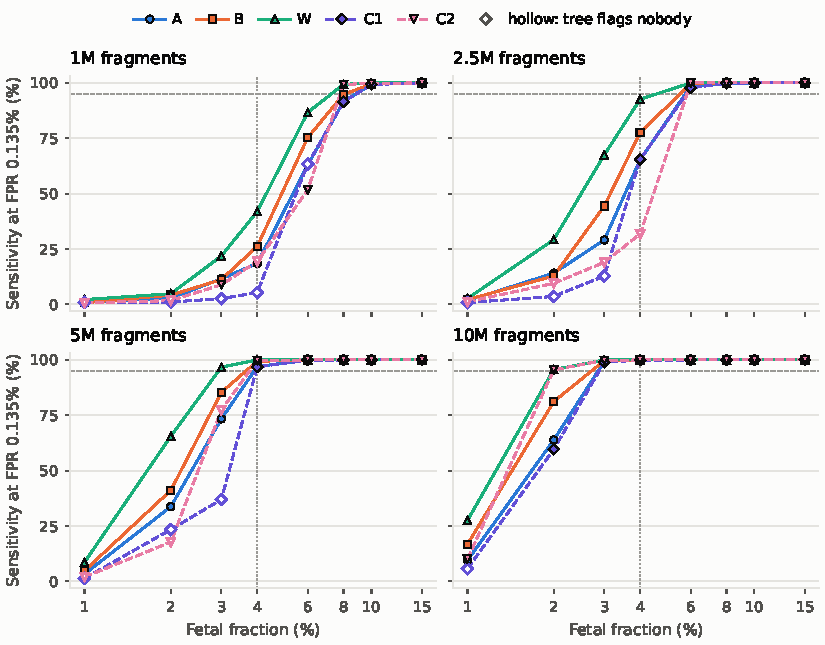
\includegraphics[width=\textwidth]{../results/figures/figS1_methods_none.pdf}
\caption{As Fig. 5, at no noise ($\sigma = 0\%$).}
\label{fig:figS1_methods_none}
\end{figure}

\begin{figure}[p]
\centering
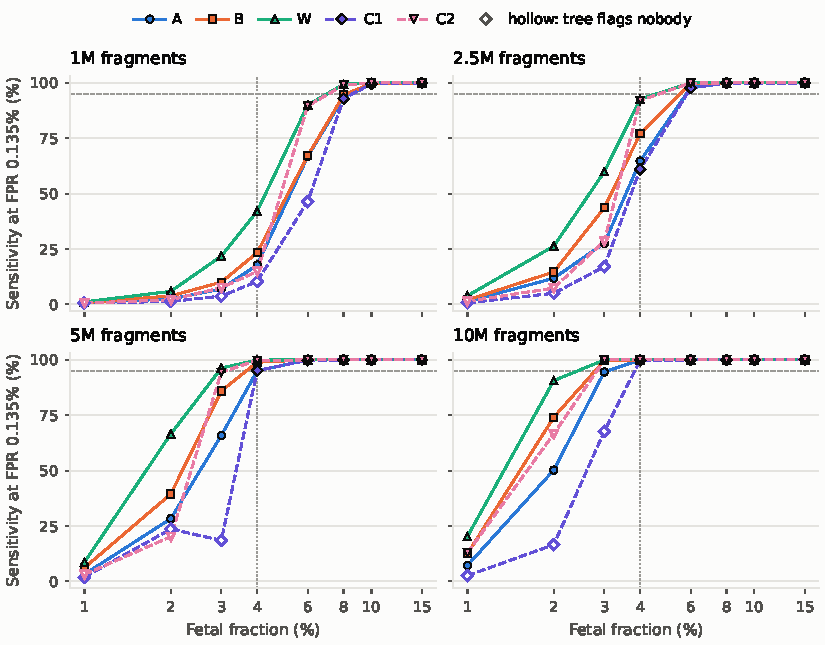
\includegraphics[width=\textwidth]{../results/figures/figS2_methods_low.pdf}
\caption{As Fig. 5, at low noise ($\sigma = 0.15\%$).}
\label{fig:figS2_methods_low}
\end{figure}

\begin{figure}[p]
\centering
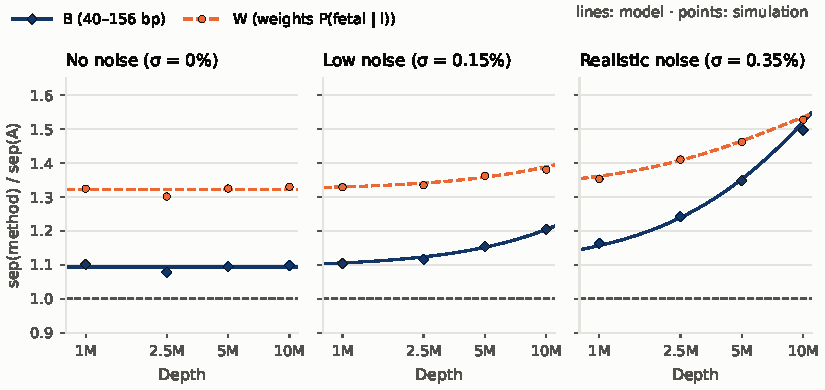
\includegraphics[width=\textwidth]{../results/figures/figS3_unified_model.pdf}
\caption{One counting model for size selection and length weighting, FF 4\%: ratio of standardised separations sep(method)/sep(A) for B (40--156\,bp) and W (each fragment weighted by $P(\mathrm{fetal} \mid \mathrm{length})$ at the true FF). Points: simulation; lines: the unified model, in which every z-score method is a chr21 fraction with length weights $u(l)$, and the break-even formula (see Methods) holds with an effective enrichment $g_\mathrm{eff} = E[u w^*]/(\mathrm{FF}\cdot E[u])$ and an effective read fraction $r_\mathrm{eff} = E[u]^2/E[u^2]$. Dashed: method = A. Like W, the model uses the true length distributions.}
\label{fig:figS3_unified_model}
\end{figure}

\begin{figure}[p]
\centering
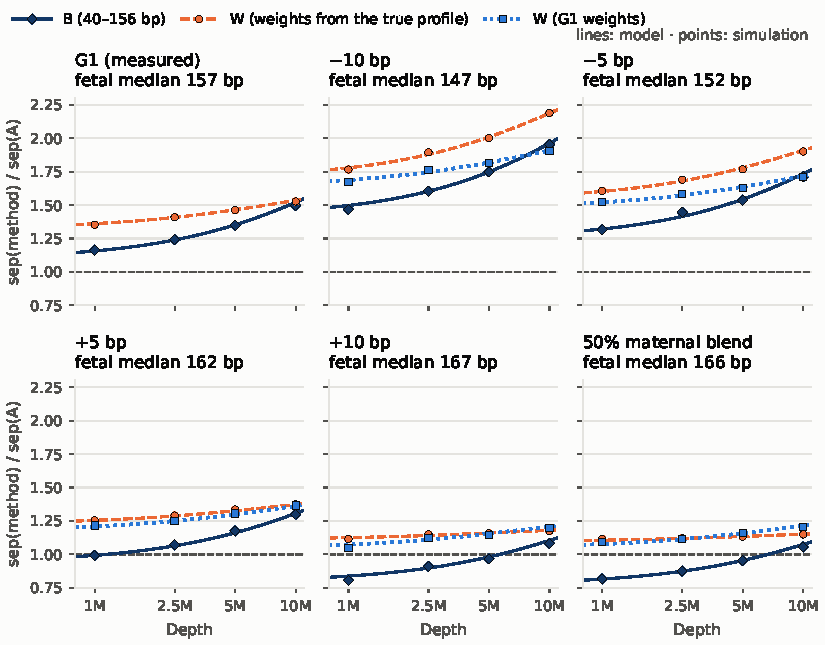
\includegraphics[width=\textwidth]{../results/figures/figS4_profiles.pdf}
\caption{Gain over A under different fetal length profiles, FF 4\%, realistic noise ($\sigma = 0.35\%$): ratio of standardised separations sep(method)/sep(A) for B (40--156\,bp), W (weights $P(\mathrm{fetal} \mid \mathrm{length})$ from the patients' true profile) and W (G1 weights) (weights from G1 (measured), the profile used in the main analysis, as a lab using a published profile would; in G1 (measured) it equals W). Scenarios shift the fetal length distribution by $-$10 to +10\,bp (fetal median 147\,bp, 152\,bp, 157\,bp, 162\,bp, 167\,bp for shifts of $-$10, $-$5, +0, +5, +10\,bp; maternal 172\,bp) or blend it 50:50 with the maternal one (50\% maternal blend, fetal median 166\,bp); all groups, including the reference, are simulated from the scenario profile. Points: simulation; lines: the unified counting model (Fig. S3) with each method's weights and the scenario's true length distributions. Dashed: method = A.}
\label{fig:figS4_profiles}
\end{figure}

\begin{figure}[p]
\centering
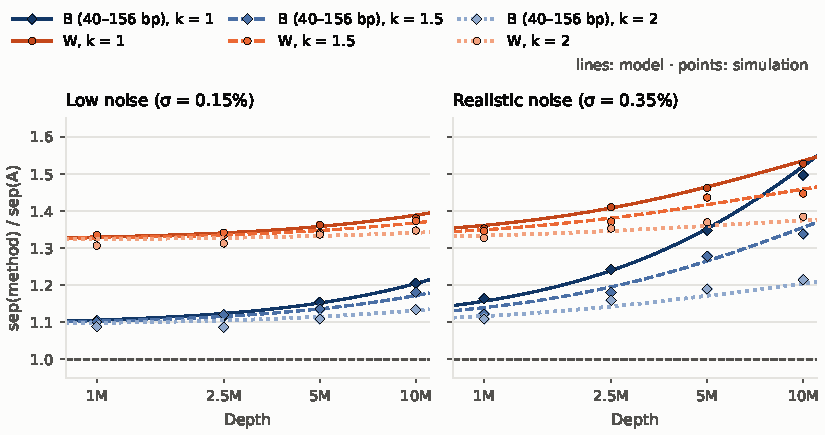
\includegraphics[width=\textwidth]{../results/figures/figS5_short_noise.pdf}
\caption{Gain over A with extra noise on short fragments, FF 4\%: ratio of standardised separations sep(method)/sep(A) for B (40--156\,bp) and W, at $k = 1$ (main analysis), 1.5 and 2. In the $k$ scenarios each patient's chr21 fragments of 40--156\,bp get a second, independent relative noise $\sigma_s = \sigma\sqrt{k^2 - 1}$, so the window's chr21 fraction has relative SD $\approx \sigma k$ (a step at 156\,bp, the worst case for B); all groups, including the reference, are simulated with it. Points: simulation; lines: the counting model with $\sigma_u^2 = \sigma^2 + \sigma_s^2 \rho_u^2$, $\rho_u$ the share of a method's weight inside the window (A: 0.20, B: 1, W: 0.49 at FF 4\%), so $\sigma_B/\sigma_A = 1.46$ ($k = 1.5$) and 1.89 ($k = 2$). Dashed: method = A.}
\label{fig:figS5_short_noise}
\end{figure}

\clearpage
\section*{Supplementary tables}

% Table S1. Generated by python -m src.evaluate.latex_tables from tableS1_bopt_cutoff.csv; do not edit.
{\footnotesize
\begin{longtable}{@{}llrrrrrrrr@{}}
\caption{B-opt: upper cutoff chosen per condition on the training set (grid 120--170\,bp in 5\,bp steps, lower bound 40\,bp; see Methods), with its training separation, and B-opt vs B (40--156\,bp) on the test set: standardised separation, sensitivity at FPR 0.135\% and the difference B-opt $-$ B (points).}\label{tab:s1} \\
\toprule
Noise & Depth & FF (\%) & \begin{tabular}[b]{@{}c@{}}Cutoff\\(bp)\end{tabular} & \begin{tabular}[b]{@{}c@{}}Sep.\\train\end{tabular} & \begin{tabular}[b]{@{}c@{}}Sep.\\B-opt\end{tabular} & \begin{tabular}[b]{@{}c@{}}Sep.\\B\end{tabular} & \begin{tabular}[b]{@{}c@{}}Sens.\ (\%)\\B-opt\end{tabular} & \begin{tabular}[b]{@{}c@{}}Sens.\ (\%)\\B\end{tabular} & \begin{tabular}[b]{@{}c@{}}Diff.\\(pts)\end{tabular} \\
\midrule
\endfirsthead
\multicolumn{10}{l}{\emph{(continued)}} \\
\toprule
Noise & Depth & FF (\%) & \begin{tabular}[b]{@{}c@{}}Cutoff\\(bp)\end{tabular} & \begin{tabular}[b]{@{}c@{}}Sep.\\train\end{tabular} & \begin{tabular}[b]{@{}c@{}}Sep.\\B-opt\end{tabular} & \begin{tabular}[b]{@{}c@{}}Sep.\\B\end{tabular} & \begin{tabular}[b]{@{}c@{}}Sens.\ (\%)\\B-opt\end{tabular} & \begin{tabular}[b]{@{}c@{}}Sens.\ (\%)\\B\end{tabular} & \begin{tabular}[b]{@{}c@{}}Diff.\\(pts)\end{tabular} \\
\midrule
\endhead
\bottomrule
\endfoot
no noise & 1M & 1 & 160 & 0.61 & 0.60 & 0.60 & 1.0 & 0.7 & +0.3 \\
no noise & 1M & 2 & 155 & 1.21 & 1.24 & 1.24 & 5.0 & 4.2 & +0.8 \\
no noise & 1M & 3 & 160 & 1.81 & 1.82 & 1.83 & 14.4 & 11.2 & +3.2 \\
no noise & 1M & 4 & 160 & 2.46 & 2.40 & 2.43 & 26.6 & 26.2 & +0.4 \\
no noise & 1M & 6 & 160 & 3.61 & 3.59 & 3.61 & 69.8 & 75.3 & $-$5.5 \\
no noise & 1M & 8 & 160 & 4.67 & 4.77 & 4.78 & 95.0 & 94.8 & +0.2 \\
no noise & 1M & 10 & 160 & 5.79 & 5.82 & 5.83 & 99.6 & 99.5 & +0.1 \\
no noise & 1M & 15 & 165 & 8.44 & 8.38 & 8.41 & 100.0 & 100.0 & +0.0 \\
no noise & 2.5M & 1 & 160 & 0.95 & 0.98 & 0.98 & 1.8 & 2.1 & $-$0.4 \\
no noise & 2.5M & 2 & 155 & 1.98 & 1.96 & 1.95 & 13.2 & 12.8 & +0.4 \\
no noise & 2.5M & 3 & 155 & 2.85 & 2.93 & 2.94 & 48.0 & 44.4 & +3.6 \\
no noise & 2.5M & 4 & 160 & 3.86 & 3.82 & 3.82 & 78.6 & 77.6 & +0.9 \\
no noise & 2.5M & 6 & 155 & 5.62 & 5.61 & 5.62 & 99.5 & 99.6 & $-$0.1 \\
no noise & 2.5M & 8 & 160 & 7.56 & 7.42 & 7.45 & 100.0 & 100.0 & +0.0 \\
no noise & 2.5M & 10 & 160 & 9.19 & 9.37 & 9.25 & 100.0 & 100.0 & +0.0 \\
no noise & 2.5M & 15 & 165 & 13.54 & 13.55 & 13.37 & 100.0 & 100.0 & +0.0 \\
no noise & 5M & 1 & 155 & 1.37 & 1.34 & 1.35 & 4.0 & 4.8 & $-$0.8 \\
no noise & 5M & 2 & 155 & 2.72 & 2.78 & 2.78 & 42.9 & 41.1 & +1.8 \\
no noise & 5M & 3 & 155 & 4.02 & 4.09 & 4.10 & 85.2 & 85.4 & $-$0.1 \\
no noise & 5M & 4 & 160 & 5.46 & 5.46 & 5.48 & 99.0 & 99.4 & $-$0.4 \\
no noise & 5M & 6 & 160 & 7.92 & 7.96 & 7.94 & 100.0 & 100.0 & +0.0 \\
no noise & 5M & 8 & 155 & 10.66 & 10.54 & 10.54 & 100.0 & 100.0 & +0.0 \\
no noise & 5M & 10 & 160 & 13.13 & 13.05 & 13.02 & 100.0 & 100.0 & +0.0 \\
no noise & 5M & 15 & 165 & 19.02 & 19.04 & 18.90 & 100.0 & 100.0 & +0.0 \\
no noise & 10M & 1 & 155 & 1.98 & 1.97 & 1.98 & 15.4 & 16.7 & $-$1.2 \\
no noise & 10M & 2 & 155 & 3.93 & 3.86 & 3.87 & 84.5 & 81.2 & +3.4 \\
no noise & 10M & 3 & 155 & 5.80 & 5.73 & 5.75 & 99.6 & 99.7 & $-$0.1 \\
no noise & 10M & 4 & 160 & 7.65 & 7.63 & 7.67 & 100.0 & 100.0 & +0.0 \\
no noise & 10M & 6 & 160 & 11.34 & 11.47 & 11.40 & 100.0 & 100.0 & +0.0 \\
no noise & 10M & 8 & 155 & 14.77 & 15.14 & 15.15 & 100.0 & 100.0 & +0.0 \\
no noise & 10M & 10 & 160 & 18.59 & 18.40 & 18.26 & 100.0 & 100.0 & +0.0 \\
no noise & 10M & 15 & 165 & 27.00 & 26.67 & 26.41 & 100.0 & 100.0 & +0.0 \\
low noise & 1M & 1 & 155 & 0.60 & 0.62 & 0.62 & 0.6 & 0.8 & $-$0.1 \\
low noise & 1M & 2 & 155 & 1.22 & 1.25 & 1.25 & 3.8 & 3.8 & +0.0 \\
low noise & 1M & 3 & 160 & 1.80 & 1.79 & 1.81 & 9.1 & 10.0 & $-$0.9 \\
low noise & 1M & 4 & 155 & 2.41 & 2.43 & 2.42 & 27.8 & 23.4 & +4.4 \\
low noise & 1M & 6 & 155 & 3.59 & 3.57 & 3.57 & 70.0 & 67.1 & +2.9 \\
low noise & 1M & 8 & 160 & 4.67 & 4.73 & 4.75 & 94.0 & 94.5 & $-$0.5 \\
low noise & 1M & 10 & 160 & 5.81 & 5.83 & 5.78 & 99.6 & 99.9 & $-$0.2 \\
low noise & 1M & 15 & 160 & 8.33 & 8.47 & 8.39 & 100.0 & 100.0 & +0.0 \\
low noise & 2.5M & 1 & 160 & 0.93 & 0.93 & 0.95 & 1.4 & 1.9 & $-$0.5 \\
low noise & 2.5M & 2 & 155 & 1.95 & 1.99 & 1.99 & 16.6 & 14.6 & +2.0 \\
low noise & 2.5M & 3 & 155 & 2.87 & 2.85 & 2.85 & 40.6 & 43.6 & $-$3.0 \\
low noise & 2.5M & 4 & 155 & 3.86 & 3.79 & 3.80 & 78.3 & 77.0 & +1.3 \\
low noise & 2.5M & 6 & 155 & 5.57 & 5.60 & 5.63 & 99.5 & 99.6 & $-$0.1 \\
low noise & 2.5M & 8 & 155 & 7.45 & 7.38 & 7.41 & 100.0 & 100.0 & +0.0 \\
low noise & 2.5M & 10 & 160 & 9.26 & 9.15 & 9.15 & 100.0 & 100.0 & +0.0 \\
low noise & 2.5M & 15 & 160 & 13.33 & 13.19 & 13.10 & 100.0 & 100.0 & +0.0 \\
low noise & 5M & 1 & 155 & 1.34 & 1.41 & 1.41 & 7.5 & 6.1 & +1.5 \\
low noise & 5M & 2 & 155 & 2.67 & 2.69 & 2.70 & 39.4 & 39.5 & $-$0.1 \\
low noise & 5M & 3 & 155 & 4.00 & 4.10 & 4.11 & 86.2 & 86.0 & +0.2 \\
low noise & 5M & 4 & 155 & 5.27 & 5.36 & 5.35 & 99.0 & 99.0 & +0.0 \\
low noise & 5M & 6 & 155 & 7.89 & 7.95 & 7.97 & 100.0 & 100.0 & +0.0 \\
low noise & 5M & 8 & 160 & 10.43 & 10.41 & 10.44 & 100.0 & 100.0 & +0.0 \\
low noise & 5M & 10 & 160 & 12.57 & 12.74 & 12.80 & 100.0 & 100.0 & +0.0 \\
low noise & 5M & 15 & 160 & 18.71 & 18.50 & 18.36 & 100.0 & 100.0 & +0.0 \\
low noise & 10M & 1 & 155 & 1.89 & 1.93 & 1.93 & 15.0 & 12.4 & +2.5 \\
low noise & 10M & 2 & 155 & 3.76 & 3.73 & 3.74 & 73.5 & 74.1 & $-$0.6 \\
low noise & 10M & 3 & 155 & 5.49 & 5.66 & 5.66 & 99.7 & 99.8 & $-$0.1 \\
low noise & 10M & 4 & 155 & 7.57 & 7.45 & 7.47 & 100.0 & 100.0 & +0.0 \\
low noise & 10M & 6 & 155 & 10.84 & 10.94 & 10.97 & 100.0 & 100.0 & +0.0 \\
low noise & 10M & 8 & 155 & 14.28 & 14.58 & 14.64 & 100.0 & 100.0 & +0.0 \\
low noise & 10M & 10 & 160 & 17.76 & 17.93 & 17.86 & 100.0 & 100.0 & +0.0 \\
low noise & 10M & 15 & 160 & 26.01 & 26.17 & 25.95 & 100.0 & 100.0 & +0.0 \\
realistic noise & 1M & 1 & 145 & 0.63 & 0.56 & 0.57 & 0.9 & 1.1 & $-$0.1 \\
realistic noise & 1M & 2 & 160 & 1.20 & 1.20 & 1.20 & 2.9 & 2.5 & +0.4 \\
realistic noise & 1M & 3 & 150 & 1.82 & 1.83 & 1.83 & 11.8 & 9.0 & +2.7 \\
realistic noise & 1M & 4 & 155 & 2.38 & 2.37 & 2.38 & 25.6 & 23.8 & +1.8 \\
realistic noise & 1M & 6 & 155 & 3.46 & 3.50 & 3.52 & 62.8 & 66.9 & $-$4.1 \\
realistic noise & 1M & 8 & 155 & 4.59 & 4.63 & 4.64 & 93.5 & 94.2 & $-$0.6 \\
realistic noise & 1M & 10 & 160 & 5.72 & 5.76 & 5.76 & 99.4 & 99.4 & +0.0 \\
realistic noise & 1M & 15 & 160 & 8.43 & 8.33 & 8.25 & 100.0 & 100.0 & +0.0 \\
realistic noise & 2.5M & 1 & 150 & 0.89 & 0.95 & 0.96 & 1.7 & 1.4 & +0.3 \\
realistic noise & 2.5M & 2 & 155 & 1.94 & 1.93 & 1.93 & 11.5 & 14.6 & $-$3.2 \\
realistic noise & 2.5M & 3 & 155 & 2.78 & 2.80 & 2.79 & 45.6 & 43.0 & +2.6 \\
realistic noise & 2.5M & 4 & 155 & 3.64 & 3.65 & 3.65 & 73.9 & 72.7 & +1.2 \\
realistic noise & 2.5M & 6 & 155 & 5.44 & 5.39 & 5.40 & 99.2 & 99.0 & +0.2 \\
realistic noise & 2.5M & 8 & 160 & 7.05 & 7.08 & 7.19 & 100.0 & 100.0 & +0.0 \\
realistic noise & 2.5M & 10 & 160 & 8.89 & 8.71 & 8.77 & 100.0 & 100.0 & +0.0 \\
realistic noise & 2.5M & 15 & 160 & 12.88 & 12.87 & 12.90 & 100.0 & 100.0 & +0.0 \\
realistic noise & 5M & 1 & 145 & 1.32 & 1.25 & 1.25 & 4.5 & 4.2 & +0.3 \\
realistic noise & 5M & 2 & 150 & 2.54 & 2.58 & 2.54 & 36.4 & 36.0 & +0.4 \\
realistic noise & 5M & 3 & 150 & 3.86 & 3.84 & 3.84 & 78.5 & 79.2 & $-$0.8 \\
realistic noise & 5M & 4 & 155 & 5.08 & 5.09 & 5.09 & 97.9 & 98.1 & $-$0.2 \\
realistic noise & 5M & 6 & 155 & 7.39 & 7.43 & 7.42 & 100.0 & 100.0 & +0.0 \\
realistic noise & 5M & 8 & 155 & 9.66 & 9.79 & 9.79 & 100.0 & 100.0 & +0.0 \\
realistic noise & 5M & 10 & 155 & 11.97 & 11.96 & 11.99 & 100.0 & 100.0 & +0.0 \\
realistic noise & 5M & 15 & 155 & 17.55 & 17.34 & 17.32 & 100.0 & 100.0 & +0.0 \\
realistic noise & 10M & 1 & 145 & 1.71 & 1.80 & 1.72 & 12.3 & 8.1 & +4.3 \\
realistic noise & 10M & 2 & 145 & 3.48 & 3.49 & 3.43 & 60.0 & 65.8 & $-$5.9 \\
realistic noise & 10M & 3 & 150 & 5.25 & 5.17 & 5.07 & 98.2 & 97.8 & +0.4 \\
realistic noise & 10M & 4 & 150 & 6.73 & 6.80 & 6.68 & 100.0 & 100.0 & +0.0 \\
realistic noise & 10M & 6 & 150 & 9.86 & 9.95 & 9.89 & 100.0 & 100.0 & +0.0 \\
realistic noise & 10M & 8 & 150 & 13.16 & 13.06 & 12.93 & 100.0 & 100.0 & +0.0 \\
realistic noise & 10M & 10 & 155 & 15.90 & 15.64 & 15.60 & 100.0 & 100.0 & +0.0 \\
realistic noise & 10M & 15 & 155 & 22.78 & 22.85 & 22.80 & 100.0 & 100.0 & +0.0 \\
\end{longtable}
}

\clearpage

% Table S2. Generated by python -m src.evaluate.latex_tables from tableS2_c2_importances.csv; do not edit.
{\footnotesize
\begin{longtable}{@{}llrrrrrl@{}}
\caption{C2 feature importances (scikit-learn impurity importance) of $z_A$, $z_\text{short}$ and $z_W$, chosen max depth and whether the tree's threshold flags nobody, per condition.}\label{tab:s2} \\
\toprule
Noise & Depth & FF (\%) & $z_A$ & $z_\text{short}$ & $z_W$ & Max depth & Flags nobody \\
\midrule
\endfirsthead
\multicolumn{8}{l}{\emph{(continued)}} \\
\toprule
Noise & Depth & FF (\%) & $z_A$ & $z_\text{short}$ & $z_W$ & Max depth & Flags nobody \\
\midrule
\endhead
\bottomrule
\endfoot
no noise & 1M & 1 & 0.012 & 0.000 & 0.988 & 3 & yes \\
no noise & 1M & 2 & 0.000 & 0.000 & 1.000 & 3 & yes \\
no noise & 1M & 3 & 0.004 & 0.001 & 0.995 & 4 & no \\
no noise & 1M & 4 & 0.003 & 0.000 & 0.997 & 4 & yes \\
no noise & 1M & 6 & 0.000 & 0.000 & 1.000 & 3 & no \\
no noise & 1M & 8 & 0.000 & 0.000 & 1.000 & 3 & no \\
no noise & 1M & 10 & 0.000 & 0.000 & 1.000 & 3 & no \\
no noise & 1M & 15 & 0.000 & 0.000 & 1.000 & 3 & no \\
no noise & 2.5M & 1 & 0.000 & 0.000 & 1.000 & 3 & yes \\
no noise & 2.5M & 2 & 0.000 & 0.000 & 1.000 & 3 & yes \\
no noise & 2.5M & 3 & 0.000 & 0.000 & 1.000 & 3 & yes \\
no noise & 2.5M & 4 & 0.000 & 0.002 & 0.998 & 3 & yes \\
no noise & 2.5M & 6 & 0.000 & 0.001 & 0.999 & 3 & no \\
no noise & 2.5M & 8 & 0.000 & 0.000 & 1.000 & 3 & no \\
no noise & 2.5M & 10 & 0.000 & 0.000 & 1.000 & 3 & no \\
no noise & 2.5M & 15 & 0.000 & 1.000 & 0.000 & 3 & no \\
no noise & 5M & 1 & 0.000 & 0.000 & 1.000 & 3 & yes \\
no noise & 5M & 2 & 0.000 & 0.001 & 0.999 & 3 & yes \\
no noise & 5M & 3 & 0.001 & 0.001 & 0.999 & 3 & yes \\
no noise & 5M & 4 & 0.000 & 0.000 & 1.000 & 3 & no \\
no noise & 5M & 6 & 0.000 & 0.000 & 1.000 & 3 & no \\
no noise & 5M & 8 & 0.000 & 0.000 & 1.000 & 3 & no \\
no noise & 5M & 10 & 0.000 & 1.000 & 0.000 & 3 & no \\
no noise & 5M & 15 & 0.000 & 1.000 & 0.000 & 3 & no \\
no noise & 10M & 1 & 0.001 & 0.005 & 0.995 & 4 & no \\
no noise & 10M & 2 & 0.001 & 0.000 & 0.999 & 3 & no \\
no noise & 10M & 3 & 0.000 & 0.000 & 1.000 & 3 & no \\
no noise & 10M & 4 & 0.000 & 0.000 & 1.000 & 3 & no \\
no noise & 10M & 6 & 0.000 & 1.000 & 0.000 & 3 & no \\
no noise & 10M & 8 & 0.000 & 1.000 & 0.000 & 3 & no \\
no noise & 10M & 10 & 0.000 & 1.000 & 0.000 & 3 & no \\
no noise & 10M & 15 & 0.000 & 1.000 & 0.000 & 3 & no \\
low noise & 1M & 1 & 0.000 & 0.016 & 0.984 & 3 & yes \\
low noise & 1M & 2 & 0.000 & 0.000 & 1.000 & 3 & yes \\
low noise & 1M & 3 & 0.004 & 0.004 & 0.992 & 4 & yes \\
low noise & 1M & 4 & 0.000 & 0.000 & 1.000 & 3 & yes \\
low noise & 1M & 6 & 0.001 & 0.000 & 0.999 & 3 & no \\
low noise & 1M & 8 & 0.000 & 0.001 & 0.999 & 3 & no \\
low noise & 1M & 10 & 0.001 & 0.000 & 0.999 & 3 & no \\
low noise & 1M & 15 & 0.000 & 0.000 & 1.000 & 3 & no \\
low noise & 2.5M & 1 & 0.006 & 0.000 & 0.994 & 3 & yes \\
low noise & 2.5M & 2 & 0.000 & 0.000 & 1.000 & 3 & yes \\
low noise & 2.5M & 3 & 0.002 & 0.000 & 0.998 & 3 & yes \\
low noise & 2.5M & 4 & 0.000 & 0.003 & 0.997 & 4 & no \\
low noise & 2.5M & 6 & 0.000 & 0.001 & 0.999 & 3 & no \\
low noise & 2.5M & 8 & 0.000 & 0.000 & 1.000 & 3 & no \\
low noise & 2.5M & 10 & 0.000 & 0.000 & 1.000 & 3 & no \\
low noise & 2.5M & 15 & 0.000 & 0.000 & 1.000 & 3 & no \\
low noise & 5M & 1 & 0.000 & 0.000 & 1.000 & 3 & yes \\
low noise & 5M & 2 & 0.000 & 0.000 & 1.000 & 3 & yes \\
low noise & 5M & 3 & 0.000 & 0.001 & 0.999 & 3 & no \\
low noise & 5M & 4 & 0.000 & 0.000 & 1.000 & 3 & no \\
low noise & 5M & 6 & 0.000 & 0.000 & 1.000 & 3 & no \\
low noise & 5M & 8 & 0.000 & 0.000 & 1.000 & 3 & no \\
low noise & 5M & 10 & 0.000 & 1.000 & 0.000 & 3 & no \\
low noise & 5M & 15 & 0.000 & 1.000 & 0.000 & 3 & no \\
low noise & 10M & 1 & 0.007 & 0.003 & 0.991 & 4 & no \\
low noise & 10M & 2 & 0.001 & 0.001 & 0.998 & 3 & yes \\
low noise & 10M & 3 & 0.000 & 0.000 & 1.000 & 3 & no \\
low noise & 10M & 4 & 0.000 & 0.000 & 1.000 & 3 & no \\
low noise & 10M & 6 & 0.000 & 0.000 & 1.000 & 3 & no \\
low noise & 10M & 8 & 0.000 & 1.000 & 0.000 & 3 & no \\
low noise & 10M & 10 & 0.000 & 1.000 & 0.000 & 3 & no \\
low noise & 10M & 15 & 0.000 & 1.000 & 0.000 & 3 & no \\
realistic noise & 1M & 1 & 0.020 & 0.031 & 0.948 & 4 & yes \\
realistic noise & 1M & 2 & 0.000 & 0.000 & 1.000 & 3 & yes \\
realistic noise & 1M & 3 & 0.000 & 0.000 & 1.000 & 3 & yes \\
realistic noise & 1M & 4 & 0.000 & 0.000 & 1.000 & 3 & yes \\
realistic noise & 1M & 6 & 0.000 & 0.001 & 0.999 & 3 & yes \\
realistic noise & 1M & 8 & 0.000 & 0.001 & 0.999 & 3 & no \\
realistic noise & 1M & 10 & 0.000 & 0.000 & 1.000 & 3 & no \\
realistic noise & 1M & 15 & 0.000 & 0.000 & 1.000 & 3 & no \\
realistic noise & 2.5M & 1 & 0.000 & 0.000 & 1.000 & 3 & yes \\
realistic noise & 2.5M & 2 & 0.002 & 0.013 & 0.985 & 4 & no \\
realistic noise & 2.5M & 3 & 0.005 & 0.005 & 0.990 & 4 & yes \\
realistic noise & 2.5M & 4 & 0.006 & 0.002 & 0.991 & 4 & yes \\
realistic noise & 2.5M & 6 & 0.000 & 0.000 & 1.000 & 3 & no \\
realistic noise & 2.5M & 8 & 0.000 & 0.000 & 1.000 & 3 & no \\
realistic noise & 2.5M & 10 & 0.000 & 0.000 & 1.000 & 3 & no \\
realistic noise & 2.5M & 15 & 0.000 & 1.000 & 0.000 & 3 & no \\
realistic noise & 5M & 1 & 0.022 & 0.030 & 0.949 & 4 & yes \\
realistic noise & 5M & 2 & 0.017 & 0.000 & 0.983 & 3 & yes \\
realistic noise & 5M & 3 & 0.003 & 0.007 & 0.990 & 3 & no \\
realistic noise & 5M & 4 & 0.001 & 0.002 & 0.996 & 3 & no \\
realistic noise & 5M & 6 & 0.000 & 0.000 & 1.000 & 3 & no \\
realistic noise & 5M & 8 & 0.000 & 0.000 & 1.000 & 3 & no \\
realistic noise & 5M & 10 & 0.000 & 0.000 & 1.000 & 3 & no \\
realistic noise & 5M & 15 & 0.000 & 1.000 & 0.000 & 3 & no \\
realistic noise & 10M & 1 & 0.031 & 0.115 & 0.854 & 5 & yes \\
realistic noise & 10M & 2 & 0.024 & 0.019 & 0.957 & 4 & no \\
realistic noise & 10M & 3 & 0.000 & 0.008 & 0.991 & 3 & no \\
realistic noise & 10M & 4 & 0.000 & 0.000 & 1.000 & 3 & no \\
realistic noise & 10M & 6 & 0.000 & 0.000 & 1.000 & 3 & no \\
realistic noise & 10M & 8 & 0.000 & 1.000 & 0.000 & 3 & no \\
realistic noise & 10M & 10 & 0.000 & 1.000 & 0.000 & 3 & no \\
realistic noise & 10M & 15 & 0.000 & 1.000 & 0.000 & 3 & no \\
\end{longtable}
}

\clearpage

% Table S3. Generated by python -m src.evaluate.latex_tables from tableS3_w_vs_wfixed_sens.csv; do not edit.
{\scriptsize\setlength{\tabcolsep}{3pt}
\begin{longtable}{@{}llrrrrrrrr@{}}
\caption{W (weights from the true FF) vs W (FF 10\%), W with the weights fixed at FF 10\%, per condition: sensitivity at the $z > 3$ threshold, sensitivity at FPR 0.135\% (matched FPR) and AUC, and the difference W (FF 10\%) $-$ W in sensitivity at FPR 0.135\% (points).}\label{tab:s3} \\
\toprule
Noise & Depth & FF (\%) & \begin{tabular}[b]{@{}c@{}}Sens.\\W\end{tabular} & \begin{tabular}[b]{@{}c@{}}Sens.\\W (FF 10\%)\end{tabular} & \begin{tabular}[b]{@{}c@{}}Matched\\FPR W\end{tabular} & \begin{tabular}[b]{@{}c@{}}Matched\\FPR W (FF 10\%)\end{tabular} & \begin{tabular}[b]{@{}c@{}}Diff.\\(pts)\end{tabular} & \begin{tabular}[b]{@{}c@{}}AUC\\W\end{tabular} & \begin{tabular}[b]{@{}c@{}}AUC\\W (FF 10\%)\end{tabular} \\
\midrule
\endfirsthead
\multicolumn{10}{l}{\emph{(continued)}} \\
\toprule
Noise & Depth & FF (\%) & \begin{tabular}[b]{@{}c@{}}Sens.\\W\end{tabular} & \begin{tabular}[b]{@{}c@{}}Sens.\\W (FF 10\%)\end{tabular} & \begin{tabular}[b]{@{}c@{}}Matched\\FPR W\end{tabular} & \begin{tabular}[b]{@{}c@{}}Matched\\FPR W (FF 10\%)\end{tabular} & \begin{tabular}[b]{@{}c@{}}Diff.\\(pts)\end{tabular} & \begin{tabular}[b]{@{}c@{}}AUC\\W\end{tabular} & \begin{tabular}[b]{@{}c@{}}AUC\\W (FF 10\%)\end{tabular} \\
\midrule
\endhead
\bottomrule
\endfoot
no noise & 1M & 1 & 2.2 & 2.1 & 2.1 & 2.1 & $-$0.1 & 0.6972 & 0.6960 \\
no noise & 1M & 2 & 8.6 & 8.3 & 4.8 & 4.7 & $-$0.1 & 0.8534 & 0.8522 \\
no noise & 1M & 3 & 23.4 & 23.2 & 21.8 & 23.4 & +1.6 & 0.9379 & 0.9376 \\
no noise & 1M & 4 & 49.6 & 49.3 & 41.9 & 42.2 & +0.4 & 0.9799 & 0.9796 \\
no noise & 1M & 6 & 90.2 & 90.0 & 86.7 & 88.0 & +1.3 & 0.9984 & 0.9984 \\
no noise & 1M & 8 & 99.5 & 99.5 & 99.4 & 99.4 & +0.0 & 0.9999 & 1.0000 \\
no noise & 1M & 10 & 100.0 & 100.0 & 100.0 & 100.0 & +0.0 & 1.0000 & 1.0000 \\
no noise & 1M & 15 & 100.0 & 100.0 & 100.0 & 100.0 & +0.0 & 1.0000 & 1.0000 \\
no noise & 2.5M & 1 & 4.5 & 4.0 & 2.6 & 3.0 & +0.4 & 0.8043 & 0.8020 \\
no noise & 2.5M & 2 & 25.9 & 25.0 & 29.2 & 30.0 & +0.8 & 0.9539 & 0.9523 \\
no noise & 2.5M & 3 & 68.4 & 68.8 & 67.5 & 67.8 & +0.2 & 0.9926 & 0.9924 \\
no noise & 2.5M & 4 & 93.2 & 93.3 & 92.7 & 91.8 & $-$0.9 & 0.9992 & 0.9992 \\
no noise & 2.5M & 6 & 100.0 & 100.0 & 100.0 & 100.0 & +0.0 & 1.0000 & 1.0000 \\
no noise & 2.5M & 8 & 100.0 & 100.0 & 100.0 & 100.0 & +0.0 & 1.0000 & 1.0000 \\
no noise & 2.5M & 10 & 100.0 & 100.0 & 100.0 & 100.0 & +0.0 & 1.0000 & 1.0000 \\
no noise & 2.5M & 15 & 100.0 & 100.0 & 100.0 & 100.0 & +0.0 & 1.0000 & 1.0000 \\
no noise & 5M & 1 & 8.0 & 7.9 & 8.6 & 9.3 & +0.8 & 0.8717 & 0.8698 \\
no noise & 5M & 2 & 67.0 & 65.8 & 65.5 & 63.9 & $-$1.6 & 0.9908 & 0.9905 \\
no noise & 5M & 3 & 96.7 & 96.7 & 96.8 & 96.8 & +0.0 & 0.9994 & 0.9994 \\
no noise & 5M & 4 & 100.0 & 100.0 & 100.0 & 100.0 & +0.0 & 1.0000 & 1.0000 \\
no noise & 5M & 6 & 100.0 & 100.0 & 100.0 & 100.0 & +0.0 & 1.0000 & 1.0000 \\
no noise & 5M & 8 & 100.0 & 100.0 & 100.0 & 100.0 & +0.0 & 1.0000 & 1.0000 \\
no noise & 5M & 10 & 100.0 & 100.0 & 100.0 & 100.0 & +0.0 & 1.0000 & 1.0000 \\
no noise & 5M & 15 & 100.0 & 100.0 & 100.0 & 100.0 & +0.0 & 1.0000 & 1.0000 \\
no noise & 10M & 1 & 23.8 & 22.8 & 27.5 & 26.7 & $-$0.8 & 0.9533 & 0.9515 \\
no noise & 10M & 2 & 95.7 & 95.2 & 95.7 & 94.7 & $-$1.0 & 0.9996 & 0.9996 \\
no noise & 10M & 3 & 100.0 & 100.0 & 100.0 & 100.0 & +0.0 & 1.0000 & 1.0000 \\
no noise & 10M & 4 & 100.0 & 100.0 & 100.0 & 100.0 & +0.0 & 1.0000 & 1.0000 \\
no noise & 10M & 6 & 100.0 & 100.0 & 100.0 & 100.0 & +0.0 & 1.0000 & 1.0000 \\
no noise & 10M & 8 & 100.0 & 100.0 & 100.0 & 100.0 & +0.0 & 1.0000 & 1.0000 \\
no noise & 10M & 10 & 100.0 & 100.0 & 100.0 & 100.0 & +0.0 & 1.0000 & 1.0000 \\
no noise & 10M & 15 & 100.0 & 100.0 & 100.0 & 100.0 & +0.0 & 1.0000 & 1.0000 \\
low noise & 1M & 1 & 1.3 & 1.2 & 1.1 & 1.2 & +0.1 & 0.6978 & 0.6956 \\
low noise & 1M & 2 & 5.8 & 5.4 & 5.9 & 5.5 & $-$0.4 & 0.8514 & 0.8502 \\
low noise & 1M & 3 & 20.9 & 20.4 & 21.8 & 20.8 & $-$0.9 & 0.9331 & 0.9327 \\
low noise & 1M & 4 & 47.1 & 46.7 & 42.0 & 42.9 & +0.8 & 0.9794 & 0.9791 \\
low noise & 1M & 6 & 88.6 & 88.5 & 90.0 & 90.0 & +0.1 & 0.9990 & 0.9990 \\
low noise & 1M & 8 & 99.5 & 99.5 & 99.4 & 99.5 & +0.1 & 1.0000 & 1.0000 \\
low noise & 1M & 10 & 100.0 & 100.0 & 100.0 & 100.0 & +0.0 & 1.0000 & 1.0000 \\
low noise & 1M & 15 & 100.0 & 100.0 & 100.0 & 100.0 & +0.0 & 1.0000 & 1.0000 \\
low noise & 2.5M & 1 & 3.8 & 3.7 & 3.9 & 3.8 & $-$0.1 & 0.7891 & 0.7858 \\
low noise & 2.5M & 2 & 27.6 & 26.5 & 26.2 & 25.9 & $-$0.4 & 0.9481 & 0.9469 \\
low noise & 2.5M & 3 & 68.7 & 67.5 & 59.9 & 61.6 & +1.7 & 0.9922 & 0.9919 \\
low noise & 2.5M & 4 & 93.5 & 93.2 & 92.7 & 92.6 & $-$0.1 & 0.9989 & 0.9989 \\
low noise & 2.5M & 6 & 100.0 & 100.0 & 100.0 & 100.0 & +0.0 & 1.0000 & 1.0000 \\
low noise & 2.5M & 8 & 100.0 & 100.0 & 100.0 & 100.0 & +0.0 & 1.0000 & 1.0000 \\
low noise & 2.5M & 10 & 100.0 & 100.0 & 100.0 & 100.0 & +0.0 & 1.0000 & 1.0000 \\
low noise & 2.5M & 15 & 100.0 & 100.0 & 100.0 & 100.0 & +0.0 & 1.0000 & 1.0000 \\
low noise & 5M & 1 & 10.9 & 10.3 & 8.6 & 6.9 & $-$1.8 & 0.8780 & 0.8746 \\
low noise & 5M & 2 & 57.4 & 56.9 & 66.5 & 63.5 & $-$3.0 & 0.9877 & 0.9870 \\
low noise & 5M & 3 & 96.7 & 96.2 & 96.4 & 95.8 & $-$0.5 & 0.9997 & 0.9997 \\
low noise & 5M & 4 & 100.0 & 99.9 & 100.0 & 100.0 & +0.1 & 1.0000 & 1.0000 \\
low noise & 5M & 6 & 100.0 & 100.0 & 100.0 & 100.0 & +0.0 & 1.0000 & 1.0000 \\
low noise & 5M & 8 & 100.0 & 100.0 & 100.0 & 100.0 & +0.0 & 1.0000 & 1.0000 \\
low noise & 5M & 10 & 100.0 & 100.0 & 100.0 & 100.0 & +0.0 & 1.0000 & 1.0000 \\
low noise & 5M & 15 & 100.0 & 100.0 & 100.0 & 100.0 & +0.0 & 1.0000 & 1.0000 \\
low noise & 10M & 1 & 20.4 & 19.6 & 20.2 & 18.9 & $-$1.4 & 0.9440 & 0.9405 \\
low noise & 10M & 2 & 90.8 & 89.8 & 90.6 & 90.2 & $-$0.4 & 0.9987 & 0.9985 \\
low noise & 10M & 3 & 100.0 & 100.0 & 100.0 & 100.0 & +0.0 & 1.0000 & 1.0000 \\
low noise & 10M & 4 & 100.0 & 100.0 & 100.0 & 100.0 & +0.0 & 1.0000 & 1.0000 \\
low noise & 10M & 6 & 100.0 & 100.0 & 100.0 & 100.0 & +0.0 & 1.0000 & 1.0000 \\
low noise & 10M & 8 & 100.0 & 100.0 & 100.0 & 100.0 & +0.0 & 1.0000 & 1.0000 \\
low noise & 10M & 10 & 100.0 & 100.0 & 100.0 & 100.0 & +0.0 & 1.0000 & 1.0000 \\
low noise & 10M & 15 & 100.0 & 100.0 & 100.0 & 100.0 & +0.0 & 1.0000 & 1.0000 \\
realistic noise & 1M & 1 & 1.1 & 1.0 & 1.2 & 1.0 & $-$0.2 & 0.6901 & 0.6877 \\
realistic noise & 1M & 2 & 6.7 & 6.8 & 5.2 & 4.6 & $-$0.6 & 0.8426 & 0.8407 \\
realistic noise & 1M & 3 & 18.9 & 17.9 & 17.6 & 19.1 & +1.4 & 0.9325 & 0.9304 \\
realistic noise & 1M & 4 & 41.2 & 40.0 & 40.7 & 39.9 & $-$0.8 & 0.9753 & 0.9746 \\
realistic noise & 1M & 6 & 87.0 & 86.7 & 81.9 & 82.2 & +0.2 & 0.9984 & 0.9984 \\
realistic noise & 1M & 8 & 99.1 & 99.1 & 98.7 & 98.6 & $-$0.1 & 0.9999 & 0.9999 \\
realistic noise & 1M & 10 & 100.0 & 100.0 & 100.0 & 100.0 & +0.0 & 1.0000 & 1.0000 \\
realistic noise & 1M & 15 & 100.0 & 100.0 & 100.0 & 100.0 & +0.0 & 1.0000 & 1.0000 \\
realistic noise & 2.5M & 1 & 3.1 & 2.9 & 1.7 & 1.2 & $-$0.5 & 0.7794 & 0.7745 \\
realistic noise & 2.5M & 2 & 19.7 & 18.9 & 17.9 & 17.5 & $-$0.4 & 0.9351 & 0.9317 \\
realistic noise & 2.5M & 3 & 61.3 & 59.1 & 59.9 & 59.0 & $-$0.9 & 0.9871 & 0.9860 \\
realistic noise & 2.5M & 4 & 87.6 & 86.4 & 85.9 & 84.9 & $-$1.0 & 0.9981 & 0.9978 \\
realistic noise & 2.5M & 6 & 100.0 & 99.9 & 100.0 & 100.0 & +0.0 & 1.0000 & 1.0000 \\
realistic noise & 2.5M & 8 & 100.0 & 100.0 & 100.0 & 100.0 & +0.0 & 1.0000 & 1.0000 \\
realistic noise & 2.5M & 10 & 100.0 & 100.0 & 100.0 & 100.0 & +0.0 & 1.0000 & 1.0000 \\
realistic noise & 2.5M & 15 & 100.0 & 100.0 & 100.0 & 100.0 & +0.0 & 1.0000 & 1.0000 \\
realistic noise & 5M & 1 & 6.1 & 5.6 & 7.1 & 6.9 & $-$0.3 & 0.8322 & 0.8245 \\
realistic noise & 5M & 2 & 43.9 & 41.0 & 43.0 & 40.6 & $-$2.4 & 0.9785 & 0.9758 \\
realistic noise & 5M & 3 & 86.1 & 84.4 & 87.7 & 86.6 & $-$1.1 & 0.9979 & 0.9974 \\
realistic noise & 5M & 4 & 99.0 & 98.7 & 99.6 & 99.2 & $-$0.4 & 0.9999 & 0.9999 \\
realistic noise & 5M & 6 & 100.0 & 100.0 & 100.0 & 100.0 & +0.0 & 1.0000 & 1.0000 \\
realistic noise & 5M & 8 & 100.0 & 100.0 & 100.0 & 100.0 & +0.0 & 1.0000 & 1.0000 \\
realistic noise & 5M & 10 & 100.0 & 100.0 & 100.0 & 100.0 & +0.0 & 1.0000 & 1.0000 \\
realistic noise & 5M & 15 & 100.0 & 100.0 & 100.0 & 100.0 & +0.0 & 1.0000 & 1.0000 \\
realistic noise & 10M & 1 & 13.1 & 11.2 & 10.4 & 10.0 & $-$0.4 & 0.8962 & 0.8853 \\
realistic noise & 10M & 2 & 67.0 & 62.6 & 64.8 & 60.0 & $-$4.8 & 0.9919 & 0.9896 \\
realistic noise & 10M & 3 & 98.5 & 97.2 & 98.0 & 96.9 & $-$1.1 & 0.9998 & 0.9997 \\
realistic noise & 10M & 4 & 100.0 & 100.0 & 100.0 & 100.0 & +0.0 & 1.0000 & 1.0000 \\
realistic noise & 10M & 6 & 100.0 & 100.0 & 100.0 & 100.0 & +0.0 & 1.0000 & 1.0000 \\
realistic noise & 10M & 8 & 100.0 & 100.0 & 100.0 & 100.0 & +0.0 & 1.0000 & 1.0000 \\
realistic noise & 10M & 10 & 100.0 & 100.0 & 100.0 & 100.0 & +0.0 & 1.0000 & 1.0000 \\
realistic noise & 10M & 15 & 100.0 & 100.0 & 100.0 & 100.0 & +0.0 & 1.0000 & 1.0000 \\
\end{longtable}
}

\clearpage

% Table S4. Generated by python -m src.evaluate.latex_tables from tableS4_w_vs_wfixed_limits.csv; do not edit.
\begin{table}[htbp]
\centering
\small
\caption{Detection limits of W (weights from the true FF) and W (FF 10\%) (weights fixed at FF 10\%) per depth and noise level (own threshold and conservative, on the 14-point FF grid (1, 1.5, 2, 2.5, 3, 3.5, 4, 5, 6, 7, 8, 9, 10, 15\%) as in Table 2), and the difference W (FF 10\%) $-$ W of the own-threshold limits (FF points).}
\label{tab:s4}
\smallskip
\begin{tabular}{@{}llrrrrr@{}}
\toprule
Noise & Depth & W & W (FF 10\%) & W (cons.) & W (FF 10\%) (cons.) & Diff.\ (pts) \\
\midrule
no noise & 1M & 6.62 & 6.63 & 6.74 & 6.75 & +0.01 \\
no noise & 2.5M & 4.27 & 4.25 & 4.39 & 4.38 & $-$0.01 \\
no noise & 5M & 2.91 & 2.92 & 2.96 & 2.96 & +0.01 \\
no noise & 10M & 1.98 & 2.00 & 2.03 & 2.08 & +0.01 \\
low noise & 1M & 6.72 & 6.73 & 6.83 & 6.83 & +0.01 \\
low noise & 2.5M & 4.27 & 4.29 & 4.42 & 4.44 & +0.03 \\
low noise & 5M & 2.94 & 2.96 & 2.97 & 2.99 & +0.02 \\
low noise & 10M & 2.24 & 2.27 & 2.28 & 2.32 & +0.04 \\
realistic noise & 1M & 6.90 & 6.93 & 7.03 & 7.09 & +0.02 \\
realistic noise & 2.5M & 4.70 & 4.76 & 4.78 & 4.84 & +0.06 \\
realistic noise & 5M & 3.39 & 3.45 & 3.43 & 3.49 & +0.05 \\
realistic noise & 10M & 2.77 & 2.88 & 2.83 & 2.93 & +0.12 \\
\bottomrule
\end{tabular}
\end{table}

\clearpage

% Table S5. Generated by python -m src.evaluate.latex_tables from tableS5_auc.csv; do not edit.
{\scriptsize\setlength{\tabcolsep}{3pt}
\begin{longtable}{@{}llrrrrrrrr@{}}
\caption{AUC of the test ROC (10,000 euploid and 2,000 trisomic test patients per condition) per condition of the 8-point FF grid of the simulated conditions (1, 2, 3, 4, 6, 8, 10, 15\%). AUC values for the main methods; all cutoffs in the repository (tableS5\_auc.csv).}\label{tab:s5} \\
\toprule
Noise & Depth & FF (\%) & A & B & B-opt & W & W (FF 10\%) & C1 & C2 \\
\midrule
\endfirsthead
\multicolumn{10}{l}{\emph{(continued)}} \\
\toprule
Noise & Depth & FF (\%) & A & B & B-opt & W & W (FF 10\%) & C1 & C2 \\
\midrule
\endhead
\bottomrule
\endfoot
no noise & 1M & 1 & 0.6509 & 0.6644 & 0.6641 & 0.6972 & 0.6960 & 0.6423 & 0.6817 \\
no noise & 1M & 2 & 0.7841 & 0.8075 & 0.8054 & 0.8534 & 0.8522 & 0.7773 & 0.8483 \\
no noise & 1M & 3 & 0.8800 & 0.8994 & 0.8964 & 0.9379 & 0.9376 & 0.8742 & 0.9306 \\
no noise & 1M & 4 & 0.9388 & 0.9541 & 0.9524 & 0.9799 & 0.9796 & 0.9333 & 0.9765 \\
no noise & 1M & 6 & 0.9905 & 0.9939 & 0.9936 & 0.9984 & 0.9984 & 0.9860 & 0.9964 \\
no noise & 1M & 8 & 0.9992 & 0.9995 & 0.9996 & 0.9999 & 1.0000 & 0.9980 & 0.9993 \\
no noise & 1M & 10 & 1.0000 & 1.0000 & 1.0000 & 1.0000 & 1.0000 & 0.9991 & 0.9994 \\
no noise & 1M & 15 & 1.0000 & 1.0000 & 1.0000 & 1.0000 & 1.0000 & 1.0000 & 1.0000 \\
no noise & 2.5M & 1 & 0.7337 & 0.7547 & 0.7552 & 0.8043 & 0.8020 & 0.7281 & 0.7992 \\
no noise & 2.5M & 2 & 0.8879 & 0.9152 & 0.9163 & 0.9539 & 0.9523 & 0.8845 & 0.9496 \\
no noise & 2.5M & 3 & 0.9669 & 0.9784 & 0.9781 & 0.9926 & 0.9924 & 0.9647 & 0.9879 \\
no noise & 2.5M & 4 & 0.9935 & 0.9962 & 0.9956 & 0.9992 & 0.9992 & 0.9926 & 0.9938 \\
no noise & 2.5M & 6 & 0.9999 & 1.0000 & 1.0000 & 1.0000 & 1.0000 & 0.9985 & 0.9997 \\
no noise & 2.5M & 8 & 1.0000 & 1.0000 & 1.0000 & 1.0000 & 1.0000 & 0.9991 & 1.0000 \\
no noise & 2.5M & 10 & 1.0000 & 1.0000 & 1.0000 & 1.0000 & 1.0000 & 1.0000 & 1.0000 \\
no noise & 2.5M & 15 & 1.0000 & 1.0000 & 1.0000 & 1.0000 & 1.0000 & 1.0000 & 1.0000 \\
no noise & 5M & 1 & 0.7950 & 0.8298 & 0.8302 & 0.8717 & 0.8698 & 0.7889 & 0.8642 \\
no noise & 5M & 2 & 0.9604 & 0.9750 & 0.9747 & 0.9908 & 0.9905 & 0.9570 & 0.9869 \\
no noise & 5M & 3 & 0.9956 & 0.9969 & 0.9968 & 0.9994 & 0.9994 & 0.9917 & 0.9963 \\
no noise & 5M & 4 & 0.9998 & 0.9999 & 0.9999 & 1.0000 & 1.0000 & 0.9992 & 0.9990 \\
no noise & 5M & 6 & 1.0000 & 1.0000 & 1.0000 & 1.0000 & 1.0000 & 0.9998 & 1.0000 \\
no noise & 5M & 8 & 1.0000 & 1.0000 & 1.0000 & 1.0000 & 1.0000 & 1.0000 & 1.0000 \\
no noise & 5M & 10 & 1.0000 & 1.0000 & 1.0000 & 1.0000 & 1.0000 & 1.0000 & 1.0000 \\
no noise & 5M & 15 & 1.0000 & 1.0000 & 1.0000 & 1.0000 & 1.0000 & 1.0000 & 1.0000 \\
no noise & 10M & 1 & 0.8844 & 0.9189 & 0.9174 & 0.9533 & 0.9515 & 0.8802 & 0.9500 \\
no noise & 10M & 2 & 0.9934 & 0.9971 & 0.9970 & 0.9996 & 0.9996 & 0.9911 & 0.9992 \\
no noise & 10M & 3 & 0.9999 & 1.0000 & 1.0000 & 1.0000 & 1.0000 & 0.9996 & 0.9992 \\
no noise & 10M & 4 & 1.0000 & 1.0000 & 1.0000 & 1.0000 & 1.0000 & 0.9996 & 1.0000 \\
no noise & 10M & 6 & 1.0000 & 1.0000 & 1.0000 & 1.0000 & 1.0000 & 1.0000 & 1.0000 \\
no noise & 10M & 8 & 1.0000 & 1.0000 & 1.0000 & 1.0000 & 1.0000 & 1.0000 & 1.0000 \\
no noise & 10M & 10 & 1.0000 & 1.0000 & 1.0000 & 1.0000 & 1.0000 & 1.0000 & 1.0000 \\
no noise & 10M & 15 & 1.0000 & 1.0000 & 1.0000 & 1.0000 & 1.0000 & 1.0000 & 1.0000 \\
low noise & 1M & 1 & 0.6437 & 0.6707 & 0.6711 & 0.6978 & 0.6956 & 0.6401 & 0.6911 \\
low noise & 1M & 2 & 0.7764 & 0.8138 & 0.8142 & 0.8514 & 0.8502 & 0.7731 & 0.8442 \\
low noise & 1M & 3 & 0.8753 & 0.8948 & 0.8930 & 0.9331 & 0.9327 & 0.8710 & 0.9278 \\
low noise & 1M & 4 & 0.9383 & 0.9534 & 0.9541 & 0.9794 & 0.9791 & 0.9371 & 0.9763 \\
low noise & 1M & 6 & 0.9903 & 0.9944 & 0.9944 & 0.9990 & 0.9990 & 0.9892 & 0.9977 \\
low noise & 1M & 8 & 0.9990 & 0.9996 & 0.9996 & 1.0000 & 1.0000 & 0.9979 & 0.9995 \\
low noise & 1M & 10 & 1.0000 & 1.0000 & 1.0000 & 1.0000 & 1.0000 & 0.9995 & 1.0000 \\
low noise & 1M & 15 & 1.0000 & 1.0000 & 1.0000 & 1.0000 & 1.0000 & 1.0000 & 1.0000 \\
low noise & 2.5M & 1 & 0.7132 & 0.7484 & 0.7434 & 0.7891 & 0.7858 & 0.7082 & 0.7819 \\
low noise & 2.5M & 2 & 0.8844 & 0.9171 & 0.9161 & 0.9481 & 0.9469 & 0.8826 & 0.9415 \\
low noise & 2.5M & 3 & 0.9633 & 0.9775 & 0.9780 & 0.9922 & 0.9919 & 0.9614 & 0.9877 \\
low noise & 2.5M & 4 & 0.9897 & 0.9957 & 0.9955 & 0.9989 & 0.9989 & 0.9854 & 0.9953 \\
low noise & 2.5M & 6 & 0.9998 & 1.0000 & 0.9999 & 1.0000 & 1.0000 & 0.9959 & 0.9995 \\
low noise & 2.5M & 8 & 1.0000 & 1.0000 & 1.0000 & 1.0000 & 1.0000 & 0.9999 & 1.0000 \\
low noise & 2.5M & 10 & 1.0000 & 1.0000 & 1.0000 & 1.0000 & 1.0000 & 0.9998 & 1.0000 \\
low noise & 2.5M & 15 & 1.0000 & 1.0000 & 1.0000 & 1.0000 & 1.0000 & 1.0000 & 1.0000 \\
low noise & 5M & 1 & 0.7970 & 0.8374 & 0.8383 & 0.8780 & 0.8746 & 0.7894 & 0.8732 \\
low noise & 5M & 2 & 0.9485 & 0.9711 & 0.9710 & 0.9877 & 0.9870 & 0.9461 & 0.9837 \\
low noise & 5M & 3 & 0.9926 & 0.9982 & 0.9983 & 0.9997 & 0.9997 & 0.9878 & 0.9978 \\
low noise & 5M & 4 & 0.9996 & 0.9999 & 0.9999 & 1.0000 & 1.0000 & 0.9988 & 0.9994 \\
low noise & 5M & 6 & 1.0000 & 1.0000 & 1.0000 & 1.0000 & 1.0000 & 0.9992 & 1.0000 \\
low noise & 5M & 8 & 1.0000 & 1.0000 & 1.0000 & 1.0000 & 1.0000 & 1.0000 & 1.0000 \\
low noise & 5M & 10 & 1.0000 & 1.0000 & 1.0000 & 1.0000 & 1.0000 & 1.0000 & 1.0000 \\
low noise & 5M & 15 & 1.0000 & 1.0000 & 1.0000 & 1.0000 & 1.0000 & 1.0000 & 1.0000 \\
low noise & 10M & 1 & 0.8642 & 0.9147 & 0.9152 & 0.9440 & 0.9405 & 0.8584 & 0.9409 \\
low noise & 10M & 2 & 0.9833 & 0.9958 & 0.9957 & 0.9987 & 0.9985 & 0.9790 & 0.9955 \\
low noise & 10M & 3 & 0.9993 & 1.0000 & 1.0000 & 1.0000 & 1.0000 & 0.9978 & 0.9999 \\
low noise & 10M & 4 & 1.0000 & 1.0000 & 1.0000 & 1.0000 & 1.0000 & 0.9995 & 1.0000 \\
low noise & 10M & 6 & 1.0000 & 1.0000 & 1.0000 & 1.0000 & 1.0000 & 1.0000 & 1.0000 \\
low noise & 10M & 8 & 1.0000 & 1.0000 & 1.0000 & 1.0000 & 1.0000 & 1.0000 & 1.0000 \\
low noise & 10M & 10 & 1.0000 & 1.0000 & 1.0000 & 1.0000 & 1.0000 & 1.0000 & 1.0000 \\
low noise & 10M & 15 & 1.0000 & 1.0000 & 1.0000 & 1.0000 & 1.0000 & 1.0000 & 1.0000 \\
realistic noise & 1M & 1 & 0.6419 & 0.6547 & 0.6522 & 0.6901 & 0.6877 & 0.6360 & 0.6802 \\
realistic noise & 1M & 2 & 0.7702 & 0.7984 & 0.7986 & 0.8426 & 0.8407 & 0.7639 & 0.8365 \\
realistic noise & 1M & 3 & 0.8568 & 0.8992 & 0.9007 & 0.9325 & 0.9304 & 0.8525 & 0.9285 \\
realistic noise & 1M & 4 & 0.9266 & 0.9549 & 0.9537 & 0.9753 & 0.9746 & 0.9241 & 0.9708 \\
realistic noise & 1M & 6 & 0.9869 & 0.9935 & 0.9932 & 0.9984 & 0.9984 & 0.9803 & 0.9967 \\
realistic noise & 1M & 8 & 0.9980 & 0.9994 & 0.9994 & 0.9999 & 0.9999 & 0.9966 & 0.9987 \\
realistic noise & 1M & 10 & 0.9999 & 1.0000 & 0.9999 & 1.0000 & 1.0000 & 0.9998 & 0.9987 \\
realistic noise & 1M & 15 & 1.0000 & 1.0000 & 1.0000 & 1.0000 & 1.0000 & 1.0000 & 1.0000 \\
realistic noise & 2.5M & 1 & 0.7025 & 0.7483 & 0.7459 & 0.7794 & 0.7745 & 0.6979 & 0.7756 \\
realistic noise & 2.5M & 2 & 0.8566 & 0.9093 & 0.9097 & 0.9351 & 0.9317 & 0.8533 & 0.9317 \\
realistic noise & 2.5M & 3 & 0.9438 & 0.9744 & 0.9743 & 0.9871 & 0.9860 & 0.9376 & 0.9842 \\
realistic noise & 2.5M & 4 & 0.9806 & 0.9949 & 0.9950 & 0.9981 & 0.9978 & 0.9749 & 0.9937 \\
realistic noise & 2.5M & 6 & 0.9991 & 1.0000 & 0.9999 & 1.0000 & 1.0000 & 0.9962 & 0.9987 \\
realistic noise & 2.5M & 8 & 1.0000 & 1.0000 & 1.0000 & 1.0000 & 1.0000 & 0.9989 & 1.0000 \\
realistic noise & 2.5M & 10 & 1.0000 & 1.0000 & 1.0000 & 1.0000 & 1.0000 & 0.9999 & 1.0000 \\
realistic noise & 2.5M & 15 & 1.0000 & 1.0000 & 1.0000 & 1.0000 & 1.0000 & 1.0000 & 0.9998 \\
realistic noise & 5M & 1 & 0.7355 & 0.8136 & 0.8116 & 0.8322 & 0.8245 & 0.7324 & 0.8325 \\
realistic noise & 5M & 2 & 0.9129 & 0.9676 & 0.9695 & 0.9785 & 0.9758 & 0.9109 & 0.9744 \\
realistic noise & 5M & 3 & 0.9751 & 0.9961 & 0.9955 & 0.9979 & 0.9974 & 0.9703 & 0.9938 \\
realistic noise & 5M & 4 & 0.9962 & 0.9998 & 0.9998 & 0.9999 & 0.9999 & 0.9947 & 0.9988 \\
realistic noise & 5M & 6 & 1.0000 & 1.0000 & 1.0000 & 1.0000 & 1.0000 & 0.9997 & 1.0000 \\
realistic noise & 5M & 8 & 1.0000 & 1.0000 & 1.0000 & 1.0000 & 1.0000 & 0.9997 & 1.0000 \\
realistic noise & 5M & 10 & 1.0000 & 1.0000 & 1.0000 & 1.0000 & 1.0000 & 1.0000 & 1.0000 \\
realistic noise & 5M & 15 & 1.0000 & 1.0000 & 1.0000 & 1.0000 & 1.0000 & 1.0000 & 1.0000 \\
realistic noise & 10M & 1 & 0.7819 & 0.8872 & 0.8952 & 0.8962 & 0.8853 & 0.7741 & 0.9044 \\
realistic noise & 10M & 2 & 0.9402 & 0.9908 & 0.9923 & 0.9919 & 0.9896 & 0.9378 & 0.9900 \\
realistic noise & 10M & 3 & 0.9890 & 0.9999 & 0.9999 & 0.9998 & 0.9997 & 0.9847 & 0.9973 \\
realistic noise & 10M & 4 & 0.9988 & 1.0000 & 1.0000 & 1.0000 & 1.0000 & 0.9972 & 0.9997 \\
realistic noise & 10M & 6 & 1.0000 & 1.0000 & 1.0000 & 1.0000 & 1.0000 & 0.9992 & 1.0000 \\
realistic noise & 10M & 8 & 1.0000 & 1.0000 & 1.0000 & 1.0000 & 1.0000 & 1.0000 & 1.0000 \\
realistic noise & 10M & 10 & 1.0000 & 1.0000 & 1.0000 & 1.0000 & 1.0000 & 1.0000 & 1.0000 \\
realistic noise & 10M & 15 & 1.0000 & 1.0000 & 1.0000 & 1.0000 & 1.0000 & 1.0000 & 1.0000 \\
\end{longtable}
}

\clearpage

% Table S6. Generated by python -m src.evaluate.latex_tables from tableS6_limits_conservative_fpr.csv; do not edit.
{\footnotesize
\begin{longtable}{@{}llrr@{}}
\caption{Detection limits on the 14-point FF grid (1, 1.5, 2, 2.5, 3, 3.5, 4, 5, 6, 7, 8, 9, 10, 15\%): conservative estimate from the Wilson 95\% lower bound of each sensitivity (plain values, no CI), and the matched-FPR limit from the sensitivity at FPR 0.135\% read from the test ROC, which compares all methods at the same FPR, with its 95\% CI (test + reference for z-score methods, test for trees).}\label{tab:s6} \\
\toprule
Depth & Method & Conservative & Matched FPR [95\% CI] \\
\midrule
\endfirsthead
\multicolumn{4}{l}{\emph{(continued)}} \\
\toprule
Depth & Method & Conservative & Matched FPR [95\% CI] \\
\midrule
\endhead
\bottomrule
\endfoot
\addlinespace
\multicolumn{4}{l}{\emph{No noise}} \\
1M & A & 8.79 & 8.72 [8.46--9.09] \\
1M & B & 8.00 & 8.05 [7.74--8.52] \\
1M & B-opt & 8.05 & 7.99 [7.84--8.44] \\
1M & W & 6.74 & 6.73 [6.51--6.86] \\
1M & C1 & 9.13 & 8.73 [8.49--9.66] \\
1M & C2 & 6.99 & 6.95 [6.85--8.83] \\
2.5M & A & 5.66 & 5.23 [4.98--5.53] \\
2.5M & B & 4.98 & 4.97 [4.91--5.27] \\
2.5M & B-opt & 4.99 & 4.94 [4.86--5.23] \\
2.5M & W & 4.39 & 4.33 [4.13--4.52] \\
2.5M & C1 & 5.98 & 5.48 [5.11--6.24] \\
2.5M & C2 & 5.95 & 4.93 [4.91--4.94] \\
5M & A & 3.87 & 3.85 [3.72--3.94] \\
5M & B & 3.49 & 3.44 [3.39--3.53] \\
5M & B-opt & 3.49 & 3.45 [3.40--3.60] \\
5M & W & 2.96 & 2.91 [2.84--3.04] \\
5M & C1 & 4.00 & 3.98 [3.93--4.86] \\
5M & C2 & 3.49 & 3.39 [2.95--3.45] \\
10M & A & 2.82 & 2.75 [2.63--2.82] \\
10M & B & 2.49 & 2.46 [2.42--2.62] \\
10M & B-opt & 2.48 & 2.49 [2.42--2.63] \\
10M & W & 2.03 & 1.99 [1.96--2.25] \\
10M & C1 & 2.99 & 2.92 [2.69--2.96] \\
10M & C2 & 2.10 & 2.00 [1.99--2.43] \\
\addlinespace
\multicolumn{4}{l}{\emph{Low noise}} \\
1M & A & 8.78 & 8.38 [7.97--8.80] \\
1M & B & 8.06 & 8.15 [7.88--8.47] \\
1M & B-opt & 8.29 & 8.27 [7.82--8.57] \\
1M & W & 6.83 & 6.59 [6.35--6.73] \\
1M & C1 & 9.96 & 8.48 [8.23--9.76] \\
1M & C2 & 6.86 & 6.61 [6.47--8.10] \\
2.5M & A & 5.73 & 5.73 [5.62--5.81] \\
2.5M & B & 5.11 & 5.12 [4.91--5.57] \\
2.5M & B-opt & 5.18 & 4.96 [4.91--5.33] \\
2.5M & W & 4.42 & 4.36 [4.10--4.50] \\
2.5M & C1 & 5.98 & 5.96 [5.94--5.97] \\
2.5M & C2 & 4.96 & 4.41 [4.28--4.77] \\
5M & A & 4.44 & 3.99 [3.91--4.18] \\
5M & B & 3.63 & 3.43 [3.37--3.57] \\
5M & B-opt & 3.68 & 3.52 [3.41--3.64] \\
5M & W & 2.97 & 2.95 [2.90--3.08] \\
5M & C1 & 4.29 & 4.00 [3.98--4.82] \\
5M & C2 & 3.29 & 3.06 [2.99--3.18] \\
10M & A & 3.07 & 3.04 [2.96--3.14] \\
10M & B & 2.53 & 2.58 [2.45--2.64] \\
10M & B-opt & 2.53 & 2.54 [2.46--2.65] \\
10M & W & 2.28 & 2.24 [2.04--2.35] \\
10M & C1 & 3.48 & 3.43 [2.98--3.46] \\
10M & C2 & 2.48 & 2.43 [2.09--2.46] \\
\addlinespace
\multicolumn{4}{l}{\emph{Realistic noise}} \\
1M & A & 9.31 & 9.40 [8.95--9.66] \\
1M & B & 8.42 & 8.24 [7.89--8.66] \\
1M & B-opt & 8.55 & 8.37 [7.88--8.56] \\
1M & W & 7.03 & 6.93 [6.74--7.29] \\
1M & C1 & 9.69 & 9.48 [9.19--9.92] \\
1M & C2 & 7.41 & 7.00 [6.97--8.30] \\
2.5M & A & 6.64 & 6.57 [6.30--6.72] \\
2.5M & B & 5.53 & 5.43 [5.14--5.69] \\
2.5M & B-opt & 5.56 & 5.39 [5.09--5.64] \\
2.5M & W & 4.78 & 4.78 [4.57--4.88] \\
2.5M & C1 & 6.83 & 6.59 [6.33--6.88] \\
2.5M & C2 & 4.97 & 4.88 [4.62--4.96] \\
5M & A & 5.32 & 5.00 [4.89--5.36] \\
5M & B & 3.80 & 3.77 [3.58--3.90] \\
5M & B-opt & 3.83 & 3.83 [3.58--3.91] \\
5M & W & 3.43 & 3.46 [3.38--3.56] \\
5M & C1 & 5.96 & 5.48 [4.97--5.90] \\
5M & C2 & 3.74 & 3.52 [3.41--3.82] \\
10M & A & 4.47 & 4.39 [4.10--4.55] \\
10M & B & 2.89 & 2.85 [2.76--2.91] \\
10M & B-opt & 2.85 & 2.82 [2.73--2.88] \\
10M & W & 2.83 & 2.84 [2.72--2.89] \\
10M & C1 & 4.76 & 4.60 [4.35--4.90] \\
10M & C2 & 2.98 & 2.97 [2.96--3.43] \\
\end{longtable}
}

\clearpage

% Table S7. Generated by python -m src.evaluate.latex_tables from tableS7_limits_8_vs_14.csv; do not edit.
{\footnotesize
\begin{longtable}{@{}llrrr@{}}
\caption{Interpolation check: detection limits on the 8-point FF grid of the simulated conditions (1, 2, 3, 4, 6, 8, 10, 15\%) (as originally reported) and on the 14-point FF grid (1, 1.5, 2, 2.5, 3, 3.5, 4, 5, 6, 7, 8, 9, 10, 15\%) (Table 2), per method and setting, and the change (points).}\label{tab:s7} \\
\toprule
Depth & Method & 8-point & 14-point & Change (pts) \\
\midrule
\endfirsthead
\multicolumn{5}{l}{\emph{(continued)}} \\
\toprule
Depth & Method & 8-point & 14-point & Change (pts) \\
\midrule
\endhead
\bottomrule
\endfoot
\addlinespace
\multicolumn{5}{l}{\emph{No noise}} \\
1M & A & 8.94 & 8.65 & $-$0.30 \\
1M & B & 7.92 & 7.89 & $-$0.03 \\
1M & B-opt & 7.93 & 7.90 & $-$0.03 \\
1M & W & 7.03 & 6.62 & $-$0.41 \\
1M & C1 & 9.03 & 8.87 & $-$0.16 \\
1M & C2 & 7.91 & 6.98 & $-$0.93 \\
1M & W (FF 10\%) & 7.05 & 6.63 & $-$0.42 \\
2.5M & A & 5.78 & 5.54 & $-$0.24 \\
2.5M & B & 5.61 & 4.94 & $-$0.67 \\
2.5M & B-opt & 5.61 & 4.95 & $-$0.66 \\
2.5M & W & 4.52 & 4.27 & $-$0.25 \\
2.5M & C1 & 5.84 & 5.97 & +0.14 \\
2.5M & C2 & 5.90 & 5.95 & +0.05 \\
2.5M & W (FF 10\%) & 4.50 & 4.25 & $-$0.24 \\
5M & A & 3.90 & 3.77 & $-$0.13 \\
5M & B & 3.74 & 3.46 & $-$0.28 \\
5M & B-opt & 3.73 & 3.45 & $-$0.28 \\
5M & W & 2.94 & 2.91 & $-$0.03 \\
5M & C1 & 3.98 & 3.99 & +0.01 \\
5M & C2 & 3.95 & 3.48 & $-$0.47 \\
5M & W (FF 10\%) & 2.95 & 2.92 & $-$0.03 \\
10M & A & 2.88 & 2.76 & $-$0.12 \\
10M & B & 2.73 & 2.46 & $-$0.28 \\
10M & B-opt & 2.74 & 2.44 & $-$0.29 \\
10M & W & 1.99 & 1.98 & $-$0.01 \\
10M & C1 & 2.91 & 2.99 & +0.07 \\
10M & C2 & 2.00 & 2.00 & +0.00 \\
10M & W (FF 10\%) & 2.00 & 2.00 & $-$0.00 \\
\addlinespace
\multicolumn{5}{l}{\emph{Low noise}} \\
1M & A & 9.06 & 8.65 & $-$0.40 \\
1M & B & 7.94 & 7.90 & $-$0.04 \\
1M & B-opt & 8.04 & 8.03 & $-$0.01 \\
1M & W & 7.18 & 6.72 & $-$0.46 \\
1M & C1 & 9.38 & 9.96 & +0.58 \\
1M & C2 & 7.35 & 6.77 & $-$0.58 \\
1M & W (FF 10\%) & 7.18 & 6.73 & $-$0.45 \\
2.5M & A & 5.78 & 5.64 & $-$0.14 \\
2.5M & B & 5.49 & 4.97 & $-$0.52 \\
2.5M & B-opt & 5.51 & 4.99 & $-$0.52 \\
2.5M & W & 4.46 & 4.27 & $-$0.20 \\
2.5M & C1 & 5.87 & 5.97 & +0.10 \\
2.5M & C2 & 5.90 & 4.96 & $-$0.94 \\
2.5M & W (FF 10\%) & 4.52 & 4.29 & $-$0.22 \\
5M & A & 4.61 & 4.32 & $-$0.29 \\
5M & B & 3.70 & 3.52 & $-$0.18 \\
5M & B-opt & 3.69 & 3.59 & $-$0.10 \\
5M & W & 2.96 & 2.94 & $-$0.02 \\
5M & C1 & 4.13 & 4.08 & $-$0.06 \\
5M & C2 & 3.38 & 3.23 & $-$0.16 \\
5M & W (FF 10\%) & 2.97 & 2.96 & $-$0.01 \\
10M & A & 2.99 & 2.99 & $-$0.00 \\
10M & B & 2.77 & 2.48 & $-$0.29 \\
10M & B-opt & 2.77 & 2.48 & $-$0.29 \\
10M & W & 2.45 & 2.24 & $-$0.22 \\
10M & C1 & 3.95 & 3.48 & $-$0.47 \\
10M & C2 & 2.95 & 2.48 & $-$0.47 \\
10M & W (FF 10\%) & 2.51 & 2.27 & $-$0.24 \\
\addlinespace
\multicolumn{5}{l}{\emph{Realistic noise}} \\
1M & A & 9.42 & 8.99 & $-$0.43 \\
1M & B & 8.32 & 8.19 & $-$0.12 \\
1M & B-opt & 8.55 & 8.35 & $-$0.20 \\
1M & W & 7.33 & 6.90 & $-$0.42 \\
1M & C1 & 9.46 & 9.54 & +0.08 \\
1M & C2 & 7.94 & 7.14 & $-$0.80 \\
1M & W (FF 10\%) & 7.34 & 6.93 & $-$0.42 \\
2.5M & A & 6.86 & 6.52 & $-$0.34 \\
2.5M & B & 5.71 & 5.38 & $-$0.33 \\
2.5M & B-opt & 5.71 & 5.42 & $-$0.29 \\
2.5M & W & 5.20 & 4.70 & $-$0.50 \\
2.5M & C1 & 7.39 & 6.78 & $-$0.62 \\
2.5M & C2 & 5.90 & 4.97 & $-$0.94 \\
2.5M & W (FF 10\%) & 5.28 & 4.76 & $-$0.51 \\
5M & A & 5.61 & 5.14 & $-$0.47 \\
5M & B & 3.86 & 3.71 & $-$0.16 \\
5M & B-opt & 3.85 & 3.74 & $-$0.11 \\
5M & W & 3.69 & 3.39 & $-$0.30 \\
5M & C1 & 5.91 & 5.96 & +0.04 \\
5M & C2 & 3.72 & 3.65 & $-$0.07 \\
5M & W (FF 10\%) & 3.74 & 3.45 & $-$0.30 \\
10M & A & 4.60 & 4.33 & $-$0.26 \\
10M & B & 2.91 & 2.85 & $-$0.07 \\
10M & B-opt & 2.90 & 2.80 & $-$0.10 \\
10M & W & 2.89 & 2.77 & $-$0.12 \\
10M & C1 & 5.17 & 4.67 & $-$0.50 \\
10M & C2 & 2.80 & 2.98 & +0.18 \\
10M & W (FF 10\%) & 2.93 & 2.88 & $-$0.05 \\
\end{longtable}
}

\clearpage

% Table S8. Generated by python -m src.evaluate.latex_tables from tableS8_limit_differences.csv; do not edit.
{\footnotesize
\begin{longtable}{@{}lllrlrl@{}}
\caption{Differences between detection limits (first method minus second, FF points) on the 14-point FF grid (1, 1.5, 2, 2.5, 3, 3.5, 4, 5, 6, 7, 8, 9, 10, 15\%), with 95\% CIs: test + reference version for pairs of z-score methods, test version for pairs with a tree; own-threshold basis (each method at its own threshold, as in Table 2) and matched-FPR basis (all methods at FPR 0.135\%, Table S6). Clear: the CI excludes 0; otherwise similar. For tree pairs the own-threshold basis compares methods at different achieved FPRs and is not used on its own to call a difference clear.}\label{tab:s8} \\
\toprule
Pair & Noise & Depth & Own threshold [95\% CI] & & Matched FPR [95\% CI] & \\
\midrule
\endfirsthead
\multicolumn{7}{l}{\emph{(continued)}} \\
\toprule
Pair & Noise & Depth & Own threshold [95\% CI] & & Matched FPR [95\% CI] & \\
\midrule
\endhead
\bottomrule
\endfoot
W $-$ B & no noise & 1M & $-$1.27 [$-$1.54--$-$1.08] & clear & $-$1.31 [$-$1.83--$-$0.96] & clear \\
W $-$ B & no noise & 2.5M & $-$0.67 [$-$0.88--$-$0.52] & clear & $-$0.64 [$-$1.00--$-$0.46] & clear \\
W $-$ B & no noise & 5M & $-$0.55 [$-$0.64--$-$0.49] & clear & $-$0.53 [$-$0.64--$-$0.39] & clear \\
W $-$ B & no noise & 10M & $-$0.47 [$-$0.52--$-$0.38] & clear & $-$0.47 [$-$0.63--$-$0.22] & clear \\
W $-$ B & low noise & 1M & $-$1.17 [$-$1.43--$-$1.02] & clear & $-$1.56 [$-$1.94--$-$1.24] & clear \\
W $-$ B & low noise & 2.5M & $-$0.70 [$-$1.03--$-$0.54] & clear & $-$0.77 [$-$1.28--$-$0.48] & clear \\
W $-$ B & low noise & 5M & $-$0.58 [$-$0.74--$-$0.48] & clear & $-$0.48 [$-$0.63--$-$0.35] & clear \\
W $-$ B & low noise & 10M & $-$0.24 [$-$0.34--$-$0.18] & clear & $-$0.33 [$-$0.53--$-$0.15] & clear \\
W $-$ B & realistic noise & 1M & $-$1.29 [$-$1.60--$-$0.89] & clear & $-$1.31 [$-$1.82--$-$0.86] & clear \\
W $-$ B & realistic noise & 2.5M & $-$0.68 [$-$0.83--$-$0.47] & clear & $-$0.65 [$-$0.97--$-$0.38] & clear \\
W $-$ B & realistic noise & 5M & $-$0.31 [$-$0.39--$-$0.17] & clear & $-$0.31 [$-$0.46--$-$0.13] & clear \\
W $-$ B & realistic noise & 10M & $-$0.08 [$-$0.15--$-$0.02] & clear & $-$0.01 [$-$0.13--0.06] & similar \\
W $-$ A & no noise & 1M & $-$2.02 [$-$2.23--$-$1.79] & clear & $-$1.99 [$-$2.43--$-$1.69] & clear \\
W $-$ A & no noise & 2.5M & $-$1.27 [$-$1.52--$-$1.07] & clear & $-$0.90 [$-$1.28--$-$0.58] & clear \\
W $-$ A & no noise & 5M & $-$0.86 [$-$0.98--$-$0.67] & clear & $-$0.93 [$-$1.06--$-$0.74] & clear \\
W $-$ A & no noise & 10M & $-$0.78 [$-$0.84--$-$0.67] & clear & $-$0.76 [$-$0.83--$-$0.51] & clear \\
W $-$ A & low noise & 1M & $-$1.93 [$-$2.11--$-$1.72] & clear & $-$1.79 [$-$2.24--$-$1.34] & clear \\
W $-$ A & low noise & 2.5M & $-$1.37 [$-$1.63--$-$1.16] & clear & $-$1.37 [$-$1.63--$-$1.18] & clear \\
W $-$ A & low noise & 5M & $-$1.39 [$-$1.56--$-$1.16] & clear & $-$1.04 [$-$1.24--$-$0.90] & clear \\
W $-$ A & low noise & 10M & $-$0.75 [$-$0.87--$-$0.68] & clear & $-$0.80 [$-$1.04--$-$0.65] & clear \\
W $-$ A & realistic noise & 1M & $-$2.08 [$-$2.47--$-$1.80] & clear & $-$2.47 [$-$2.82--$-$1.90] & clear \\
W $-$ A & realistic noise & 2.5M & $-$1.82 [$-$1.98--$-$1.62] & clear & $-$1.79 [$-$2.05--$-$1.50] & clear \\
W $-$ A & realistic noise & 5M & $-$1.75 [$-$1.95--$-$1.54] & clear & $-$1.54 [$-$1.91--$-$1.39] & clear \\
W $-$ A & realistic noise & 10M & $-$1.57 [$-$1.75--$-$1.30] & clear & $-$1.55 [$-$1.77--$-$1.28] & clear \\
B $-$ A & no noise & 1M & $-$0.75 [$-$0.94--$-$0.51] & clear & $-$0.68 [$-$1.14--$-$0.14] & clear \\
B $-$ A & no noise & 2.5M & $-$0.60 [$-$0.74--$-$0.46] & clear & $-$0.26 [$-$0.57--0.11] & similar \\
B $-$ A & no noise & 5M & $-$0.31 [$-$0.42--$-$0.13] & clear & $-$0.41 [$-$0.52--$-$0.24] & clear \\
B $-$ A & no noise & 10M & $-$0.31 [$-$0.36--$-$0.23] & clear & $-$0.29 [$-$0.37--$-$0.11] & clear \\
B $-$ A & low noise & 1M & $-$0.76 [$-$0.93--$-$0.52] & clear & $-$0.23 [$-$0.71--0.27] & similar \\
B $-$ A & low noise & 2.5M & $-$0.67 [$-$0.77--$-$0.44] & clear & $-$0.60 [$-$0.85--$-$0.14] & clear \\
B $-$ A & low noise & 5M & $-$0.80 [$-$0.99--$-$0.54] & clear & $-$0.56 [$-$0.75--$-$0.41] & clear \\
B $-$ A & low noise & 10M & $-$0.51 [$-$0.63--$-$0.44] & clear & $-$0.47 [$-$0.66--$-$0.35] & clear \\
B $-$ A & realistic noise & 1M & $-$0.79 [$-$1.26--$-$0.50] & clear & $-$1.16 [$-$1.63--$-$0.48] & clear \\
B $-$ A & realistic noise & 2.5M & $-$1.14 [$-$1.38--$-$0.92] & clear & $-$1.15 [$-$1.46--$-$0.75] & clear \\
B $-$ A & realistic noise & 5M & $-$1.43 [$-$1.68--$-$1.21] & clear & $-$1.23 [$-$1.62--$-$1.04] & clear \\
B $-$ A & realistic noise & 10M & $-$1.49 [$-$1.66--$-$1.24] & clear & $-$1.54 [$-$1.73--$-$1.24] & clear \\
W $-$ C2 & no noise & 1M & $-$0.36 [$-$0.45--$-$0.29] & clear & $-$0.21 [$-$2.12--$-$0.10] & clear \\
W $-$ C2 & no noise & 2.5M & $-$1.68 [$-$1.83--$-$1.57] & clear & $-$0.60 [$-$0.81--$-$0.42] & clear \\
W $-$ C2 & no noise & 5M & $-$0.57 [$-$0.61--$-$0.54] & clear & $-$0.48 [$-$0.55--$-$0.06] & clear \\
W $-$ C2 & no noise & 10M & $-$0.02 [$-$0.07--$-$0.01] & clear & $-$0.01 [$-$0.35--0.01] & similar \\
W $-$ C2 & low noise & 1M & $-$0.05 [$-$0.07--$-$0.03] & clear & $-$0.02 [$-$1.57--0.06] & similar \\
W $-$ C2 & low noise & 2.5M & $-$0.69 [$-$0.85--$-$0.56] & clear & $-$0.06 [$-$0.33--0.01] & similar \\
W $-$ C2 & low noise & 5M & $-$0.29 [$-$0.33--$-$0.24] & clear & $-$0.11 [$-$0.18--$-$0.03] & clear \\
W $-$ C2 & low noise & 10M & $-$0.24 [$-$0.28--$-$0.21] & clear & $-$0.19 [$-$0.33--$-$0.01] & clear \\
W $-$ C2 & realistic noise & 1M & $-$0.24 [$-$0.37--$-$0.12] & clear & $-$0.07 [$-$1.43--$-$0.01] & clear \\
W $-$ C2 & realistic noise & 2.5M & $-$0.27 [$-$0.32--$-$0.22] & clear & $-$0.10 [$-$0.17--0.02] & similar \\
W $-$ C2 & realistic noise & 5M & $-$0.25 [$-$0.31--$-$0.17] & clear & $-$0.06 [$-$0.33--0.01] & similar \\
W $-$ C2 & realistic noise & 10M & $-$0.21 [$-$0.26--$-$0.17] & clear & $-$0.13 [$-$0.64--$-$0.10] & clear \\
C2 $-$ B & no noise & 1M & $-$0.91 [$-$1.01--$-$0.83] & clear & $-$1.10 [$-$1.57--0.88] & similar \\
C2 $-$ B & no noise & 2.5M & +1.01 [0.97--1.05] & clear & $-$0.04 [$-$0.34--0.03] & similar \\
C2 $-$ B & no noise & 5M & +0.03 [$-$0.01--0.05] & similar & $-$0.04 [$-$0.51--0.03] & similar \\
C2 $-$ B & no noise & 10M & $-$0.46 [$-$0.48--$-$0.37] & clear & $-$0.46 [$-$0.62--$-$0.04] & clear \\
C2 $-$ B & low noise & 1M & $-$1.13 [$-$1.27--$-$1.02] & clear & $-$1.54 [$-$1.88--$-$0.09] & clear \\
C2 $-$ B & low noise & 2.5M & $-$0.01 [$-$0.14--0.05] & similar & $-$0.71 [$-$1.16--$-$0.30] & clear \\
C2 $-$ B & low noise & 5M & $-$0.29 [$-$0.40--$-$0.22] & clear & $-$0.37 [$-$0.54--$-$0.25] & clear \\
C2 $-$ B & low noise & 10M & $-$0.00 [$-$0.04--0.02] & similar & $-$0.14 [$-$0.46--$-$0.01] & clear \\
C2 $-$ B & realistic noise & 1M & $-$1.05 [$-$1.31--$-$0.76] & clear & $-$1.24 [$-$1.65--0.05] & similar \\
C2 $-$ B & realistic noise & 2.5M & $-$0.41 [$-$0.52--$-$0.27] & clear & $-$0.55 [$-$0.93--$-$0.28] & clear \\
C2 $-$ B & realistic noise & 5M & $-$0.06 [$-$0.14--0.01] & similar & $-$0.25 [$-$0.40--0.01] & similar \\
C2 $-$ B & realistic noise & 10M & +0.13 [0.10--0.16] & clear & +0.11 [0.08--0.60] & clear \\
B-opt $-$ B & no noise & 1M & +0.01 [$-$0.12--0.14] & similar & $-$0.05 [$-$0.42--0.40] & similar \\
B-opt $-$ B & no noise & 2.5M & +0.01 [$-$0.04--0.07] & similar & $-$0.03 [$-$0.28--0.18] & similar \\
B-opt $-$ B & no noise & 5M & $-$0.00 [$-$0.03--0.02] & similar & +0.01 [$-$0.02--0.12] & similar \\
B-opt $-$ B & no noise & 10M & $-$0.01 [$-$0.03--0.01] & similar & +0.03 [$-$0.04--0.11] & similar \\
B-opt $-$ B & low noise & 1M & +0.13 [0.01--0.36] & clear & +0.12 [$-$0.39--0.44] & similar \\
B-opt $-$ B & low noise & 2.5M & +0.02 [$-$0.14--0.14] & similar & $-$0.16 [$-$0.53--0.15] & similar \\
B-opt $-$ B & low noise & 5M & +0.07 [$-$0.01--0.12] & similar & +0.09 [$-$0.03--0.18] & similar \\
B-opt $-$ B & low noise & 10M & $-$0.00 [$-$0.04--0.02] & similar & $-$0.04 [$-$0.10--0.08] & similar \\
B-opt $-$ B & realistic noise & 1M & +0.16 [0.00--0.32] & clear & +0.13 [$-$0.33--0.31] & similar \\
B-opt $-$ B & realistic noise & 2.5M & +0.04 [$-$0.06--0.12] & similar & $-$0.04 [$-$0.27--0.16] & similar \\
B-opt $-$ B & realistic noise & 5M & +0.04 [$-$0.02--0.11] & similar & +0.06 [$-$0.08--0.14] & similar \\
B-opt $-$ B & realistic noise & 10M & $-$0.05 [$-$0.09--0.01] & similar & $-$0.03 [$-$0.12--0.05] & similar \\
W (FF 10\%) $-$ W & no noise & 1M & +0.01 [$-$0.03--0.04] & similar & $-$0.04 [$-$0.07--0.05] & similar \\
W (FF 10\%) $-$ W & no noise & 2.5M & $-$0.01 [$-$0.08--0.03] & similar & +0.07 [$-$0.18--0.15] & similar \\
W (FF 10\%) $-$ W & no noise & 5M & +0.01 [$-$0.00--0.03] & similar & +0.01 [$-$0.04--0.04] & similar \\
W (FF 10\%) $-$ W & no noise & 10M & +0.01 [$-$0.01--0.05] & similar & +0.05 [$-$0.09--0.10] & similar \\
W (FF 10\%) $-$ W & low noise & 1M & +0.01 [$-$0.03--0.05] & similar & $-$0.01 [$-$0.08--0.09] & similar \\
W (FF 10\%) $-$ W & low noise & 2.5M & +0.03 [$-$0.03--0.09] & similar & +0.01 [$-$0.04--0.14] & similar \\
W (FF 10\%) $-$ W & low noise & 5M & +0.02 [$-$0.00--0.05] & similar & +0.02 [$-$0.03--0.12] & similar \\
W (FF 10\%) $-$ W & low noise & 10M & +0.04 [0.02--0.07] & clear & +0.02 [$-$0.03--0.11] & similar \\
W (FF 10\%) $-$ W & realistic noise & 1M & +0.02 [$-$0.02--0.07] & similar & +0.05 [$-$0.03--0.20] & similar \\
W (FF 10\%) $-$ W & realistic noise & 2.5M & +0.06 [0.03--0.10] & clear & +0.04 [$-$0.01--0.15] & similar \\
W (FF 10\%) $-$ W & realistic noise & 5M & +0.05 [0.02--0.08] & clear & +0.07 [0.03--0.15] & clear \\
W (FF 10\%) $-$ W & realistic noise & 10M & +0.12 [0.07--0.17] & clear & +0.08 [0.05--0.16] & clear \\
\end{longtable}
}

\clearpage

% Table S9. Generated by python -m src.evaluate.latex_tables from tableS9a_profile_inputs.csv, tableS9b_profile_b_vs_a.csv, tableS9c_profile_limits.csv, tableS9d_wg1_vs_a.csv; do not edit.
% Table S9 (fetal-profile scenarios), four parts
{\footnotesize

{\footnotesize
\begin{longtable}{@{}lrrrrrrrrrr@{}}
\caption{Fetal-profile scenarios (8-point FF grid of the simulated conditions (1, 2, 3, 4, 6, 8, 10, 15\%); all groups, including the reference, simulated from the scenario profile; see Methods): G1 (measured), the main analysis; fetal lengths shifted by $-$10, $-$5, +5 and +10\,bp; and a 50\% maternal blend. (a) Fetal median length and $g$, $r$, $g\sqrt{r}$ of the 40--156\,bp window at FF 2\%, 4\%, 10\%. (b) Conditions (of 96) where B's separation is below A's, where B $-$ A sensitivity at FPR 0.135\% is significantly negative (bootstrap), and where B-opt's separation is below A's, with B-opt's largest sensitivity loss. (c) Detection limits (own threshold) of A, B, B-opt, W (weights from the true profile), W (G1 weights) and W (FF 10\%) (G1 weights at FF 10\%); in G1 (measured), W (G1 weights) = W. (d) W (G1 weights) $-$ A with 95\% CIs (test + reference) in the +10\,bp and 50\% maternal blend scenarios, own-threshold and matched-FPR bases.}\label{tab:s9} \\
\multicolumn{11}{@{}l}{(a) Inputs of each fetal profile.} \\
\toprule
Profile & Median (bp) & $g$ 2\% & $r$ 2\% & $g\sqrt{r}$ 2\% & $g$ 4\% & $r$ 4\% & $g\sqrt{r}$ 4\% & $g$ 10\% & $r$ 10\% & $g\sqrt{r}$ 10\% \\
\midrule
\endfirsthead
\multicolumn{11}{l}{\emph{(continued)}} \\
\toprule
Profile & Median (bp) & $g$ 2\% & $r$ 2\% & $g\sqrt{r}$ 2\% & $g$ 4\% & $r$ 4\% & $g\sqrt{r}$ 4\% & $g$ 10\% & $r$ 10\% & $g\sqrt{r}$ 10\% \\
\midrule
\endhead
\bottomrule
\endfoot
G1 (measured) & 157 & 2.50 & 0.197 & 1.11 & 2.43 & 0.203 & 1.09 & 2.23 & 0.221 & 1.05 \\
$-$10\,bp & 147 & 3.24 & 0.200 & 1.45 & 3.09 & 0.209 & 1.42 & 2.74 & 0.237 & 1.33 \\
$-$5\,bp & 152 & 2.86 & 0.199 & 1.27 & 2.75 & 0.206 & 1.25 & 2.48 & 0.229 & 1.19 \\
+5\,bp & 162 & 2.14 & 0.196 & 0.95 & 2.09 & 0.200 & 0.94 & 1.96 & 0.214 & 0.91 \\
+10\,bp & 167 & 1.81 & 0.194 & 0.80 & 1.78 & 0.198 & 0.79 & 1.70 & 0.207 & 0.77 \\
50\% maternal blend & 166 & 1.76 & 0.194 & 0.78 & 1.73 & 0.197 & 0.77 & 1.66 & 0.206 & 0.75 \\
\end{longtable}
}

{\footnotesize
\addtocounter{table}{-1}
\begin{longtable}{@{}lrrrr@{}}
\multicolumn{5}{@{}l}{(b) B and B-opt against A (of 96 conditions).} \\[2pt]
\toprule
Profile & B $<$ A & B $-$ A sig.\ $<$ 0 & B-opt $<$ A & B-opt worst loss (pts) \\
\midrule
\endfirsthead
\multicolumn{5}{l}{\emph{(continued)}} \\
\toprule
Profile & B $<$ A & B $-$ A sig.\ $<$ 0 & B-opt $<$ A & B-opt worst loss (pts) \\
\midrule
\endhead
\bottomrule
\endfoot
G1 (measured) & 0 & 0 & 0 & $-$0.8 \\
$-$10\,bp & 0 & 0 & 0 & 0.0 \\
$-$5\,bp & 0 & 0 & 0 & 0.0 \\
+5\,bp & 61 & 10 & 59 & $-$12.0 \\
+10\,bp & 88 & 44 & 88 & $-$32.1 \\
50\% maternal blend & 88 & 45 & 88 & $-$25.2 \\
\end{longtable}
}

{\footnotesize
\addtocounter{table}{-1}
\begin{longtable}{@{}llrrrrrr@{}}
\multicolumn{8}{@{}l}{(c) Detection limits (FF, \%) per scenario.} \\[2pt]
\toprule
Noise & Depth & A & B & B-opt & W & W (G1 weights) & W (FF 10\%) \\
\midrule
\endfirsthead
\multicolumn{8}{l}{\emph{(continued)}} \\
\toprule
Noise & Depth & A & B & B-opt & W & W (G1 weights) & W (FF 10\%) \\
\midrule
\endhead
\bottomrule
\endfoot
\addlinespace
\multicolumn{8}{l}{\emph{G1 (measured)}} \\
no noise & 1M & 8.94 & 7.92 & 7.93 & 7.03 & 7.03 & 7.05 \\
no noise & 2.5M & 5.78 & 5.61 & 5.61 & 4.52 & 4.52 & 4.50 \\
no noise & 5M & 3.90 & 3.74 & 3.73 & 2.94 & 2.94 & 2.95 \\
no noise & 10M & 2.88 & 2.73 & 2.74 & 1.99 & 1.99 & 2.00 \\
low noise & 1M & 9.06 & 7.94 & 8.04 & 7.18 & 7.18 & 7.18 \\
low noise & 2.5M & 5.78 & 5.49 & 5.51 & 4.46 & 4.46 & 4.52 \\
low noise & 5M & 4.61 & 3.70 & 3.69 & 2.96 & 2.96 & 2.97 \\
low noise & 10M & 2.99 & 2.77 & 2.77 & 2.45 & 2.45 & 2.51 \\
realistic noise & 1M & 9.42 & 8.32 & 8.55 & 7.33 & 7.33 & 7.34 \\
realistic noise & 2.5M & 6.86 & 5.71 & 5.71 & 5.20 & 5.20 & 5.28 \\
realistic noise & 5M & 5.61 & 3.86 & 3.85 & 3.69 & 3.69 & 3.74 \\
realistic noise & 10M & 4.60 & 2.91 & 2.90 & 2.89 & 2.89 & 2.93 \\
\addlinespace
\multicolumn{8}{l}{\emph{$-$10\,bp}} \\
no noise & 1M & 8.79 & 6.52 & 6.57 & 5.61 & 5.70 & 5.75 \\
no noise & 2.5M & 5.74 & 3.89 & 3.85 & 3.30 & 3.49 & 3.55 \\
no noise & 5M & 3.90 & 2.85 & 2.86 & 2.47 & 2.56 & 2.64 \\
no noise & 10M & 2.86 & 1.96 & 1.95 & 1.88 & 1.89 & 1.91 \\
low noise & 1M & 8.86 & 6.52 & 6.45 & 5.65 & 5.74 & 5.77 \\
low noise & 2.5M & 5.83 & 3.93 & 3.89 & 3.39 & 3.59 & 3.65 \\
low noise & 5M & 3.98 & 2.85 & 2.81 & 2.44 & 2.63 & 2.71 \\
low noise & 10M & 3.15 & 1.97 & 1.95 & 1.90 & 1.92 & 1.94 \\
realistic noise & 1M & 9.37 & 6.77 & 6.83 & 5.75 & 5.87 & 5.90 \\
realistic noise & 2.5M & 6.76 & 3.98 & 3.97 & 3.59 & 3.80 & 3.87 \\
realistic noise & 5M & 5.60 & 2.95 & 2.85 & 2.74 & 2.89 & 2.94 \\
realistic noise & 10M & 4.86 & 2.39 & 1.97 & 1.96 & 2.37 & 2.62 \\
\addlinespace
\multicolumn{8}{l}{\emph{$-$5\,bp}} \\
no noise & 1M & 8.90 & 7.48 & 7.51 & 5.90 & 5.99 & 6.06 \\
no noise & 2.5M & 5.72 & 4.92 & 4.97 & 3.69 & 3.83 & 3.86 \\
no noise & 5M & 3.87 & 2.97 & 2.96 & 2.70 & 2.78 & 2.80 \\
no noise & 10M & 2.87 & 2.29 & 2.27 & 1.92 & 1.94 & 1.94 \\
low noise & 1M & 8.96 & 7.40 & 7.50 & 5.86 & 5.97 & 5.99 \\
low noise & 2.5M & 5.82 & 5.02 & 4.99 & 3.75 & 3.88 & 3.92 \\
low noise & 5M & 4.23 & 3.13 & 3.14 & 2.72 & 2.82 & 2.85 \\
low noise & 10M & 2.97 & 2.48 & 2.44 & 1.93 & 1.97 & 1.98 \\
realistic noise & 1M & 9.32 & 7.59 & 7.61 & 5.91 & 6.17 & 6.41 \\
realistic noise & 2.5M & 6.83 & 5.17 & 5.08 & 3.85 & 3.99 & 4.28 \\
realistic noise & 5M & 5.60 & 3.42 & 3.29 & 2.90 & 2.98 & 3.12 \\
realistic noise & 10M & 4.78 & 2.77 & 2.60 & 2.38 & 2.76 & 2.82 \\
\addlinespace
\multicolumn{8}{l}{\emph{+5\,bp}} \\
no noise & 1M & 8.84 & 9.62 & 9.48 & 7.52 & 7.72 & 7.68 \\
no noise & 2.5M & 5.78 & 5.94 & 5.88 & 5.04 & 5.26 & 5.21 \\
no noise & 5M & 3.84 & 3.98 & 3.96 & 2.98 & 3.29 & 3.25 \\
no noise & 10M & 2.89 & 2.93 & 2.92 & 2.43 & 2.65 & 2.62 \\
low noise & 1M & 8.95 & 9.55 & 9.39 & 7.58 & 7.74 & 7.74 \\
low noise & 2.5M & 5.81 & 5.93 & 5.88 & 5.23 & 5.37 & 5.37 \\
low noise & 5M & 4.00 & 4.39 & 4.17 & 3.50 & 3.63 & 3.61 \\
low noise & 10M & 2.97 & 2.96 & 2.96 & 2.71 & 2.78 & 2.78 \\
realistic noise & 1M & 9.42 & 9.77 & 9.68 & 7.79 & 7.87 & 7.87 \\
realistic noise & 2.5M & 6.85 & 6.20 & 6.33 & 5.60 & 5.66 & 5.66 \\
realistic noise & 5M & 5.62 & 4.97 & 4.86 & 3.90 & 3.94 & 3.96 \\
realistic noise & 10M & 5.08 & 3.51 & 3.61 & 3.39 & 3.41 & 3.51 \\
\addlinespace
\multicolumn{8}{l}{\emph{+10\,bp}} \\
no noise & 1M & 9.15 & 12.62 & 11.76 & 7.93 & 8.72 & 8.67 \\
no noise & 2.5M & 5.77 & 7.32 & 6.86 & 5.56 & 5.69 & 5.67 \\
no noise & 5M & 3.89 & 5.50 & 5.47 & 3.69 & 3.84 & 3.80 \\
no noise & 10M & 2.88 & 3.65 & 3.59 & 2.77 & 2.84 & 2.82 \\
low noise & 1M & 9.02 & 13.16 & 12.04 & 7.92 & 8.38 & 8.28 \\
low noise & 2.5M & 5.87 & 7.43 & 7.15 & 5.59 & 5.75 & 5.71 \\
low noise & 5M & 3.99 & 5.52 & 5.41 & 3.80 & 3.91 & 3.88 \\
low noise & 10M & 2.97 & 3.63 & 3.60 & 2.88 & 2.91 & 2.90 \\
realistic noise & 1M & 9.61 & 13.04 & 12.78 & 8.71 & 9.12 & 9.08 \\
realistic noise & 2.5M & 6.79 & 7.58 & 7.57 & 5.86 & 5.92 & 5.90 \\
realistic noise & 5M & 5.58 & 5.59 & 5.60 & 4.82 & 4.98 & 4.97 \\
realistic noise & 10M & 4.60 & 3.88 & 3.91 & 3.78 & 3.72 & 3.75 \\
\addlinespace
\multicolumn{8}{l}{\emph{50\% maternal blend}} \\
no noise & 1M & 8.90 & 12.55 & 9.82 & 7.93 & 8.25 & 8.12 \\
no noise & 2.5M & 5.80 & 7.48 & 6.71 & 5.55 & 5.64 & 5.61 \\
no noise & 5M & 3.89 & 5.46 & 5.00 & 3.72 & 3.82 & 3.79 \\
no noise & 10M & 2.88 & 3.68 & 3.21 & 2.79 & 2.83 & 2.81 \\
low noise & 1M & 9.02 & 13.17 & 10.50 & 7.94 & 8.26 & 8.23 \\
low noise & 2.5M & 5.76 & 7.54 & 6.87 & 5.58 & 5.70 & 5.67 \\
low noise & 5M & 4.55 & 5.62 & 5.29 & 3.80 & 3.87 & 3.84 \\
low noise & 10M & 3.07 & 3.74 & 3.59 & 2.88 & 2.90 & 2.89 \\
realistic noise & 1M & 9.45 & 13.15 & 10.76 & 8.59 & 8.87 & 8.83 \\
realistic noise & 2.5M & 6.68 & 7.63 & 7.33 & 5.86 & 5.87 & 5.86 \\
realistic noise & 5M & 5.66 & 5.75 & 5.72 & 5.23 & 5.04 & 5.04 \\
realistic noise & 10M & 4.92 & 3.98 & 3.96 & 3.86 & 3.75 & 3.77 \\
\end{longtable}
}

{\footnotesize
\addtocounter{table}{-1}
\begin{longtable}{@{}lllrr@{}}
\multicolumn{5}{@{}l}{(d) W (G1 weights) $-$ A (FF points, test + reference, 95\% CI).} \\[2pt]
\toprule
Scenario & Noise & Depth & Own threshold & Matched FPR \\
\midrule
\endfirsthead
\multicolumn{5}{l}{\emph{(continued)}} \\
\toprule
Scenario & Noise & Depth & Own threshold & Matched FPR \\
\midrule
\endhead
\bottomrule
\endfoot
50\% maternal blend & no noise & 1M & $-$0.64 [$-$0.99--$-$0.34] clear & $-$0.26 [$-$0.85--0.45] \\
50\% maternal blend & no noise & 2.5M & $-$0.16 [$-$0.22--$-$0.10] clear & $-$0.12 [$-$0.24--$-$0.00] clear \\
50\% maternal blend & no noise & 5M & $-$0.07 [$-$0.12--$-$0.03] clear & $-$0.14 [$-$0.24--$-$0.06] clear \\
50\% maternal blend & no noise & 10M & $-$0.05 [$-$0.08--$-$0.03] clear & $-$0.04 [$-$0.09--0.01] \\
50\% maternal blend & low noise & 1M & $-$0.76 [$-$1.09--$-$0.40] clear & $-$0.79 [$-$1.16--$-$0.18] clear \\
50\% maternal blend & low noise & 2.5M & $-$0.07 [$-$0.13--$-$0.02] clear & $-$0.15 [$-$0.23--$-$0.05] clear \\
50\% maternal blend & low noise & 5M & $-$0.68 [$-$1.00--$-$0.31] clear & $-$0.80 [$-$1.15--$-$0.18] clear \\
50\% maternal blend & low noise & 10M & $-$0.17 [$-$0.36--$-$0.08] clear & $-$0.16 [$-$0.34--$-$0.07] clear \\
50\% maternal blend & realistic noise & 1M & $-$0.59 [$-$0.90--$-$0.35] clear & $-$0.27 [$-$0.98--$-$0.07] clear \\
50\% maternal blend & realistic noise & 2.5M & $-$0.82 [$-$1.07--$-$0.36] clear & $-$0.78 [$-$1.05--$-$0.42] clear \\
50\% maternal blend & realistic noise & 5M & $-$0.62 [$-$0.82--$-$0.46] clear & $-$0.49 [$-$0.79--$-$0.33] clear \\
50\% maternal blend & realistic noise & 10M & $-$1.17 [$-$1.38--$-$0.91] clear & $-$1.14 [$-$1.37--$-$0.55] clear \\
+10\,bp & no noise & 1M & $-$0.43 [$-$0.79--$-$0.24] clear & $-$0.48 [$-$0.94--0.13] \\
+10\,bp & no noise & 2.5M & $-$0.08 [$-$0.12--$-$0.04] clear & $-$0.08 [$-$0.14--$-$0.00] clear \\
+10\,bp & no noise & 5M & $-$0.05 [$-$0.09--$-$0.00] clear & $-$0.05 [$-$0.14--0.03] \\
+10\,bp & no noise & 10M & $-$0.03 [$-$0.06--$-$0.01] clear & $-$0.02 [$-$0.09--0.02] \\
+10\,bp & low noise & 1M & $-$0.64 [$-$1.02--$-$0.34] clear & $-$1.02 [$-$1.31--$-$0.20] clear \\
+10\,bp & low noise & 2.5M & $-$0.13 [$-$0.18--$-$0.07] clear & $-$0.11 [$-$0.20--$-$0.04] clear \\
+10\,bp & low noise & 5M & $-$0.09 [$-$0.49--$-$0.03] clear & $-$0.30 [$-$0.86--0.02] \\
+10\,bp & low noise & 10M & $-$0.06 [$-$0.12--$-$0.04] clear & $-$0.09 [$-$0.55--$-$0.05] clear \\
+10\,bp & realistic noise & 1M & $-$0.49 [$-$0.74--$-$0.32] clear & $-$0.28 [$-$0.88--$-$0.01] clear \\
+10\,bp & realistic noise & 2.5M & $-$0.87 [$-$1.07--$-$0.55] clear & $-$1.05 [$-$1.38--$-$0.53] clear \\
+10\,bp & realistic noise & 5M & $-$0.60 [$-$0.80--$-$0.45] clear & $-$0.83 [$-$1.57--$-$0.55] clear \\
+10\,bp & realistic noise & 10M & $-$0.88 [$-$1.17--$-$0.50] clear & $-$0.91 [$-$1.23--$-$0.54] clear \\
\end{longtable}
}

}

\clearpage

% Table S10. Generated by python -m src.evaluate.latex_tables from tableS10a_snoise_rise.csv, tableS10b_snoise_limits.csv, tableS10c_snoise_regimes.csv; do not edit.
% Table S10 (short-fragment noise), three parts
{\footnotesize

{\scriptsize\setlength{\tabcolsep}{3pt}
\begin{longtable}{@{}llrrrrrrrr@{}}
\caption{Extra noise on the 40--156\,bp window ($k = 1$: main analysis; 8-point FF grid of the simulated conditions (1, 2, 3, 4, 6, 8, 10, 15\%), low and realistic noise; see Methods). (a) sep(B)/sep(A) at FF 4\%, 1M and 10M, simulated and model ($\sigma_u$), and the model's high-depth limit $g\sigma_A/\sigma_B$. (b) Detection limits of A, B and W. (c) The four regimes of each cutoff (B 40--$c$: window 40--$c$\,bp) by FF and $k$, from $g\sqrt{r}$ (low-depth ratio) and $g\sigma_A/\sigma_B$ (high-depth ratio), with $\sigma_A^2 = \sigma^2 + \sigma_s^2 r_\mathrm{win}^2$ and $\sigma_B^2 = \sigma^2 + \sigma_s^2 \rho_c^2$ ($r_\mathrm{win}$: fraction in the noisy window; $\rho_c = 1$ for $c \le 156$, $r_\mathrm{win}/r_c$ above): (i) B always better, (ii) worse at low depth and better at high, (iii) better at low depth and worse at high, (iv) always worse; $k_\mathrm{high}$: the $k$ where $g\sigma_A = \sigma_B$ (regime (iii) begins if $g^2 r \ge 1$); $k^*$: the $k$ above which depth no longer raises the gain.}\label{tab:s10} \\
\multicolumn{10}{@{}l}{(a) sep(B)/sep(A) at FF 4\%.} \\
\toprule
$k$ & Noise & Sim.\ 1M & Sim.\ 10M & Change (\%) & Model 1M & Model 10M & Change (\%) & $\sigma_B/\sigma_A$ & $g\sigma_A/\sigma_B$ \\
\midrule
\endfirsthead
\multicolumn{10}{l}{\emph{(continued)}} \\
\toprule
$k$ & Noise & Sim.\ 1M & Sim.\ 10M & Change (\%) & Model 1M & Model 10M & Change (\%) & $\sigma_B/\sigma_A$ & $g\sigma_A/\sigma_B$ \\
\midrule
\endhead
\bottomrule
\endfoot
1 & low noise & 1.104 & 1.205 & +9.2 & 1.106 & 1.204 & +8.9 & 1.000 & 2.426 \\
1 & realistic noise & 1.163 & 1.497 & +28.7 & 1.157 & 1.521 & +31.5 & 1.000 & 2.426 \\
1.5 & low noise & 1.101 & 1.180 & +7.2 & 1.102 & 1.172 & +6.3 & 1.463 & 1.658 \\
1.5 & realistic noise & 1.122 & 1.338 & +19.2 & 1.139 & 1.356 & +19.0 & 1.463 & 1.658 \\
2 & low noise & 1.088 & 1.134 & +4.2 & 1.098 & 1.132 & +3.1 & 1.887 & 1.286 \\
2 & realistic noise & 1.109 & 1.214 & +9.5 & 1.116 & 1.204 & +7.9 & 1.887 & 1.286 \\
\end{longtable}
}

{\footnotesize
\addtocounter{table}{-1}
\begin{longtable}{@{}lllrrr@{}}
\multicolumn{6}{@{}l}{(b) Detection limits (FF, \%) of A, B and W.} \\[2pt]
\toprule
$k$ & Noise & Depth & A & B & W \\
\midrule
\endfirsthead
\multicolumn{6}{l}{\emph{(continued)}} \\
\toprule
$k$ & Noise & Depth & A & B & W \\
\midrule
\endhead
\bottomrule
\endfoot
1 & low noise & 1M & 9.06 & 7.94 & 7.18 \\
1 & low noise & 2.5M & 5.78 & 5.49 & 4.46 \\
1 & low noise & 5M & 4.61 & 3.70 & 2.96 \\
1 & low noise & 10M & 2.99 & 2.77 & 2.45 \\
1 & realistic noise & 1M & 9.42 & 8.32 & 7.33 \\
1 & realistic noise & 2.5M & 6.86 & 5.71 & 5.20 \\
1 & realistic noise & 5M & 5.61 & 3.86 & 3.69 \\
1 & realistic noise & 10M & 4.60 & 2.91 & 2.89 \\
1.5 & low noise & 1M & 8.95 & 8.38 & 7.16 \\
1.5 & low noise & 2.5M & 5.83 & 5.62 & 4.55 \\
1.5 & low noise & 5M & 4.11 & 3.77 & 3.00 \\
1.5 & low noise & 10M & 2.96 & 2.84 & 2.53 \\
1.5 & realistic noise & 1M & 9.36 & 8.64 & 7.48 \\
1.5 & realistic noise & 2.5M & 6.79 & 5.78 & 5.38 \\
1.5 & realistic noise & 5M & 5.70 & 4.29 & 3.79 \\
1.5 & realistic noise & 10M & 4.92 & 3.45 & 2.96 \\
2 & low noise & 1M & 8.83 & 8.38 & 7.28 \\
2 & low noise & 2.5M & 5.82 & 5.66 & 4.83 \\
2 & low noise & 5M & 4.45 & 3.84 & 3.14 \\
2 & low noise & 10M & 3.18 & 2.89 & 2.67 \\
2 & realistic noise & 1M & 9.49 & 9.15 & 7.59 \\
2 & realistic noise & 2.5M & 7.03 & 5.92 & 5.42 \\
2 & realistic noise & 5M & 5.70 & 5.23 & 3.93 \\
2 & realistic noise & 10M & 5.11 & 3.88 & 3.40 \\
\end{longtable}
}

{\scriptsize\setlength{\tabcolsep}{3pt}
\addtocounter{table}{-1}
\begin{longtable}{@{}lrrrrrrrrrr@{}}
\multicolumn{11}{@{}l}{(c) Regimes per cutoff, FF and $k$.} \\[2pt]
\toprule
Method & FF (\%) & $g\sqrt{r}$ & $g^2r$ & Regime $k = 1$ & Regime $k = 1.5$ & Regime $k = 2$ & $g\sigma_A/\sigma_B$, $k = 1.5$ & $g\sigma_A/\sigma_B$, $k = 2$ & $k_\mathrm{high}$ & $k^*$ \\
\midrule
\endfirsthead
\multicolumn{11}{l}{\emph{(continued)}} \\
\toprule
Method & FF (\%) & $g\sqrt{r}$ & $g^2r$ & Regime $k = 1$ & Regime $k = 1.5$ & Regime $k = 2$ & $g\sigma_A/\sigma_B$, $k = 1.5$ & $g\sigma_A/\sigma_B$, $k = 2$ & $k_\mathrm{high}$ & $k^*$ \\
\midrule
\endhead
\bottomrule
\endfoot
B 40--120 & 1 & 0.58 & 0.34 & (ii) & (ii) & (ii) & 2.49 & 1.92 & 5.07 & -- \\
B 40--120 & 2 & 0.58 & 0.33 & (ii) & (ii) & (ii) & 2.43 & 1.88 & 4.88 & -- \\
B 40--120 & 3 & 0.57 & 0.32 & (ii) & (ii) & (ii) & 2.37 & 1.83 & 4.71 & -- \\
B 40--120 & 4 & 0.56 & 0.32 & (ii) & (ii) & (ii) & 2.31 & 1.79 & 4.55 & -- \\
B 40--120 & 6 & 0.55 & 0.30 & (ii) & (ii) & (ii) & 2.20 & 1.71 & 4.25 & -- \\
B 40--120 & 8 & 0.54 & 0.29 & (ii) & (ii) & (ii) & 2.11 & 1.64 & 4.00 & -- \\
B 40--120 & 10 & 0.52 & 0.28 & (ii) & (ii) & (ii) & 2.02 & 1.57 & 3.78 & -- \\
B 40--120 & 15 & 0.50 & 0.25 & (ii) & (ii) & (ii) & 1.83 & 1.43 & 3.31 & -- \\
B 40--130 & 1 & 0.79 & 0.62 & (ii) & (ii) & (ii) & 2.73 & 2.11 & 6.23 & 31.73 \\
B 40--130 & 2 & 0.77 & 0.60 & (ii) & (ii) & (ii) & 2.65 & 2.05 & 5.91 & 31.87 \\
B 40--130 & 3 & 0.76 & 0.58 & (ii) & (ii) & (ii) & 2.58 & 2.00 & 5.63 & 32.33 \\
B 40--130 & 4 & 0.75 & 0.57 & (ii) & (ii) & (ii) & 2.51 & 1.94 & 5.38 & 33.15 \\
B 40--130 & 6 & 0.73 & 0.54 & (ii) & (ii) & (ii) & 2.38 & 1.85 & 4.95 & 36.29 \\
B 40--130 & 8 & 0.71 & 0.51 & (ii) & (ii) & (ii) & 2.26 & 1.76 & 4.58 & 43.39 \\
B 40--130 & 10 & 0.70 & 0.49 & (ii) & (ii) & (ii) & 2.16 & 1.68 & 4.27 & 66.60 \\
B 40--130 & 15 & 0.66 & 0.43 & (ii) & (ii) & (ii) & 1.94 & 1.52 & 3.65 & -- \\
B 40--135 & 1 & 0.91 & 0.84 & (ii) & (ii) & (ii) & 2.73 & 2.11 & 6.21 & 8.09 \\
B 40--135 & 2 & 0.90 & 0.81 & (ii) & (ii) & (ii) & 2.65 & 2.05 & 5.90 & 7.98 \\
B 40--135 & 3 & 0.89 & 0.79 & (ii) & (ii) & (ii) & 2.57 & 1.99 & 5.62 & 7.87 \\
B 40--135 & 4 & 0.88 & 0.77 & (ii) & (ii) & (ii) & 2.50 & 1.94 & 5.37 & 7.78 \\
B 40--135 & 6 & 0.85 & 0.73 & (ii) & (ii) & (ii) & 2.38 & 1.85 & 4.94 & 7.60 \\
B 40--135 & 8 & 0.83 & 0.69 & (ii) & (ii) & (ii) & 2.26 & 1.76 & 4.57 & 7.46 \\
B 40--135 & 10 & 0.81 & 0.66 & (ii) & (ii) & (ii) & 2.16 & 1.68 & 4.26 & 7.33 \\
B 40--135 & 15 & 0.77 & 0.59 & (ii) & (ii) & (ii) & 1.94 & 1.52 & 3.64 & 7.11 \\
B 40--140 & 1 & 0.99 & 0.99 & (ii) & (ii) & (ii) & 2.58 & 2.00 & 5.47 & 5.54 \\
B 40--140 & 2 & 0.98 & 0.96 & (ii) & (ii) & (ii) & 2.51 & 1.94 & 5.24 & 5.47 \\
B 40--140 & 3 & 0.97 & 0.94 & (ii) & (ii) & (ii) & 2.45 & 1.90 & 5.03 & 5.41 \\
B 40--140 & 4 & 0.95 & 0.91 & (ii) & (ii) & (ii) & 2.38 & 1.85 & 4.84 & 5.34 \\
B 40--140 & 6 & 0.93 & 0.87 & (ii) & (ii) & (ii) & 2.27 & 1.76 & 4.50 & 5.23 \\
B 40--140 & 8 & 0.91 & 0.83 & (ii) & (ii) & (ii) & 2.17 & 1.69 & 4.21 & 5.13 \\
B 40--140 & 10 & 0.89 & 0.79 & (ii) & (ii) & (ii) & 2.07 & 1.62 & 3.96 & 5.03 \\
B 40--140 & 15 & 0.84 & 0.71 & (ii) & (ii) & (ii) & 1.87 & 1.47 & 3.44 & 4.84 \\
B 40--145 & 1 & 1.07 & 1.14 & (i) & (i) & (i) & 2.31 & 1.79 & 4.42 & 3.96 \\
B 40--145 & 2 & 1.06 & 1.11 & (i) & (i) & (i) & 2.26 & 1.75 & 4.29 & 3.92 \\
B 40--145 & 3 & 1.04 & 1.09 & (i) & (i) & (i) & 2.21 & 1.71 & 4.16 & 3.88 \\
B 40--145 & 4 & 1.03 & 1.06 & (i) & (i) & (i) & 2.16 & 1.68 & 4.04 & 3.84 \\
B 40--145 & 6 & 1.01 & 1.02 & (i) & (i) & (i) & 2.07 & 1.61 & 3.82 & 3.77 \\
B 40--145 & 8 & 0.99 & 0.98 & (ii) & (ii) & (ii) & 1.99 & 1.55 & 3.63 & 3.70 \\
B 40--145 & 10 & 0.97 & 0.94 & (ii) & (ii) & (ii) & 1.91 & 1.49 & 3.45 & 3.64 \\
B 40--145 & 15 & 0.92 & 0.85 & (ii) & (ii) & (ii) & 1.75 & 1.37 & 3.08 & 3.50 \\
B 40--150 & 1 & 1.10 & 1.21 & (i) & (i) & (i) & 2.04 & 1.58 & 3.61 & 3.14 \\
B 40--150 & 2 & 1.09 & 1.19 & (i) & (i) & (i) & 2.00 & 1.55 & 3.53 & 3.11 \\
B 40--150 & 3 & 1.08 & 1.16 & (i) & (i) & (i) & 1.97 & 1.52 & 3.45 & 3.09 \\
B 40--150 & 4 & 1.07 & 1.14 & (i) & (i) & (i) & 1.93 & 1.50 & 3.37 & 3.06 \\
B 40--150 & 6 & 1.05 & 1.10 & (i) & (i) & (i) & 1.86 & 1.45 & 3.23 & 3.02 \\
B 40--150 & 8 & 1.03 & 1.06 & (i) & (i) & (i) & 1.80 & 1.40 & 3.10 & 2.97 \\
B 40--150 & 10 & 1.01 & 1.03 & (i) & (i) & (i) & 1.74 & 1.36 & 2.98 & 2.93 \\
B 40--150 & 15 & 0.97 & 0.95 & (ii) & (ii) & (ii) & 1.61 & 1.26 & 2.72 & 2.83 \\
B & 1 & 1.12 & 1.25 & (i) & (i) & (i) & 1.73 & 1.34 & 2.86 & 2.48 \\
B & 2 & 1.11 & 1.23 & (i) & (i) & (i) & 1.71 & 1.32 & 2.82 & 2.46 \\
B & 3 & 1.10 & 1.21 & (i) & (i) & (i) & 1.68 & 1.30 & 2.77 & 2.45 \\
B & 4 & 1.09 & 1.20 & (i) & (i) & (i) & 1.66 & 1.29 & 2.73 & 2.43 \\
B & 6 & 1.08 & 1.16 & (i) & (i) & (i) & 1.61 & 1.25 & 2.65 & 2.40 \\
B & 8 & 1.06 & 1.13 & (i) & (i) & (i) & 1.57 & 1.22 & 2.57 & 2.38 \\
B & 10 & 1.05 & 1.10 & (i) & (i) & (i) & 1.53 & 1.19 & 2.50 & 2.35 \\
B & 15 & 1.01 & 1.03 & (i) & (i) & (i) & 1.44 & 1.13 & 2.33 & 2.29 \\
B 40--165 & 1 & 1.08 & 1.17 & (i) & (i) & (i) & 1.60 & 1.39 & 3.67 & 3.17 \\
B 40--165 & 2 & 1.08 & 1.16 & (i) & (i) & (i) & 1.58 & 1.38 & 3.61 & 3.14 \\
B 40--165 & 3 & 1.07 & 1.15 & (i) & (i) & (i) & 1.57 & 1.36 & 3.55 & 3.11 \\
B 40--165 & 4 & 1.07 & 1.14 & (i) & (i) & (i) & 1.55 & 1.35 & 3.49 & 3.08 \\
B 40--165 & 6 & 1.06 & 1.12 & (i) & (i) & (i) & 1.52 & 1.32 & 3.37 & 3.02 \\
B 40--165 & 8 & 1.05 & 1.10 & (i) & (i) & (i) & 1.49 & 1.30 & 3.26 & 2.97 \\
B 40--165 & 10 & 1.04 & 1.08 & (i) & (i) & (i) & 1.47 & 1.27 & 3.16 & 2.92 \\
B 40--165 & 15 & 1.02 & 1.04 & (i) & (i) & (i) & 1.41 & 1.22 & 2.92 & 2.80 \\
\end{longtable}
}

}

\clearpage

\end{document}
